\documentclass[a4paper]{book}
\usepackage{makeidx}
\usepackage{graphicx}
\usepackage{multicol}
\usepackage{float}
\usepackage{listings}
\usepackage{color}
\usepackage{ifthen}
\usepackage[table]{xcolor}
\usepackage{textcomp}
\usepackage{alltt}
\usepackage{ifpdf}
\ifpdf
\usepackage[pdftex,
            pagebackref=true,
            colorlinks=true,
            linkcolor=blue,
            unicode
           ]{hyperref}
\else
\usepackage[ps2pdf,
            pagebackref=true,
            colorlinks=true,
            linkcolor=blue,
            unicode
           ]{hyperref}
\usepackage{pspicture}
\fi
\usepackage[utf8]{inputenc}
\usepackage{mathptmx}
\usepackage[scaled=.90]{helvet}
\usepackage{courier}
\usepackage{doxygen}
\lstset{language=C++,inputencoding=utf8,basicstyle=\footnotesize,breaklines=true,breakatwhitespace=true,tabsize=8,numbers=left }
\makeindex
\setcounter{tocdepth}{3}
\renewcommand{\footrulewidth}{0.4pt}
\begin{document}
\hypersetup{pageanchor=false}
\begin{titlepage}
\vspace*{7cm}
\begin{center}
{\Large cryomesh-\/cute }\\
\vspace*{1cm}
{\large Generated by Doxygen 1.7.3}\\
\vspace*{0.5cm}
{\small Fri Feb 4 2011 13:02:07}\\
\end{center}
\end{titlepage}
\clearemptydoublepage
\pagenumbering{roman}
\tableofcontents
\clearemptydoublepage
\pagenumbering{arabic}
\hypersetup{pageanchor=true}
\chapter{Namespace Index}
\section{Namespace List}
Here is a list of all namespaces with brief descriptions:\begin{DoxyCompactList}
\item\contentsline{section}{\hyperlink{namespacecryomesh}{cryomesh} }{\pageref{namespacecryomesh}}{}
\item\contentsline{section}{\hyperlink{namespacecryomesh_1_1common}{cryomesh::common} }{\pageref{namespacecryomesh_1_1common}}{}
\item\contentsline{section}{\hyperlink{namespacecryomesh_1_1components}{cryomesh::components} }{\pageref{namespacecryomesh_1_1components}}{}
\end{DoxyCompactList}

\chapter{Class Index}
\section{Class Hierarchy}
This inheritance list is sorted roughly, but not completely, alphabetically:\begin{DoxyCompactList}
\item \contentsline{section}{cryomesh::common::ContainersTest}{\pageref{classcryomesh_1_1common_1_1_containers_test}}{}
\item \contentsline{section}{CoreTestsDefaults}{\pageref{class_core_tests_defaults}}{}
\item \contentsline{section}{ICuteSuite}{\pageref{class_i_cute_suite}}{}
\begin{DoxyCompactList}
\item \contentsline{section}{cryomesh::common::ConnectorTest}{\pageref{classcryomesh_1_1common_1_1_connector_test}}{}
\item \contentsline{section}{cryomesh::common::MathsTest}{\pageref{classcryomesh_1_1common_1_1_maths_test}}{}
\item \contentsline{section}{cryomesh::common::MiscTest}{\pageref{classcryomesh_1_1common_1_1_misc_test}}{}
\item \contentsline{section}{cryomesh::common::SimpleCollectionTest}{\pageref{classcryomesh_1_1common_1_1_simple_collection_test}}{}
\item \contentsline{section}{cryomesh::components::ImpulseTest}{\pageref{classcryomesh_1_1components_1_1_impulse_test}}{}
\item \contentsline{section}{cryomesh::components::NodeTest}{\pageref{classcryomesh_1_1components_1_1_node_test}}{}
\item \contentsline{section}{cryomesh::components::UseCaseImpulsePropagation}{\pageref{classcryomesh_1_1components_1_1_use_case_impulse_propagation}}{}
\end{DoxyCompactList}
\item \contentsline{section}{cryomesh::components::ImpulseCollectionTest}{\pageref{classcryomesh_1_1components_1_1_impulse_collection_test}}{}
\item \contentsline{section}{cryomesh::TestTemplates}{\pageref{classcryomesh_1_1_test_templates}}{}
\item \contentsline{section}{cryomesh::common::TimeKeeperTest}{\pageref{classcryomesh_1_1common_1_1_time_keeper_test}}{}
\end{DoxyCompactList}

\chapter{Class Index}
\section{Class List}
Here are the classes, structs, unions and interfaces with brief descriptions:\begin{DoxyCompactList}
\item\contentsline{section}{\hyperlink{classcryomesh_1_1common_1_1_connector_test}{cryomesh::common::ConnectorTest} }{\pageref{classcryomesh_1_1common_1_1_connector_test}}{}
\item\contentsline{section}{\hyperlink{classcryomesh_1_1common_1_1_containers_test}{cryomesh::common::ContainersTest} }{\pageref{classcryomesh_1_1common_1_1_containers_test}}{}
\item\contentsline{section}{\hyperlink{class_core_tests_defaults}{CoreTestsDefaults} }{\pageref{class_core_tests_defaults}}{}
\item\contentsline{section}{\hyperlink{class_i_cute_suite}{ICuteSuite} }{\pageref{class_i_cute_suite}}{}
\item\contentsline{section}{\hyperlink{classcryomesh_1_1components_1_1_impulse_collection_test}{cryomesh::components::ImpulseCollectionTest} }{\pageref{classcryomesh_1_1components_1_1_impulse_collection_test}}{}
\item\contentsline{section}{\hyperlink{classcryomesh_1_1components_1_1_impulse_test}{cryomesh::components::ImpulseTest} }{\pageref{classcryomesh_1_1components_1_1_impulse_test}}{}
\item\contentsline{section}{\hyperlink{classcryomesh_1_1common_1_1_maths_test}{cryomesh::common::MathsTest} }{\pageref{classcryomesh_1_1common_1_1_maths_test}}{}
\item\contentsline{section}{\hyperlink{classcryomesh_1_1common_1_1_misc_test}{cryomesh::common::MiscTest} }{\pageref{classcryomesh_1_1common_1_1_misc_test}}{}
\item\contentsline{section}{\hyperlink{classcryomesh_1_1components_1_1_node_test}{cryomesh::components::NodeTest} }{\pageref{classcryomesh_1_1components_1_1_node_test}}{}
\item\contentsline{section}{\hyperlink{classcryomesh_1_1common_1_1_simple_collection_test}{cryomesh::common::SimpleCollectionTest} }{\pageref{classcryomesh_1_1common_1_1_simple_collection_test}}{}
\item\contentsline{section}{\hyperlink{classcryomesh_1_1_test_templates}{cryomesh::TestTemplates} }{\pageref{classcryomesh_1_1_test_templates}}{}
\item\contentsline{section}{\hyperlink{classcryomesh_1_1common_1_1_time_keeper_test}{cryomesh::common::TimeKeeperTest} }{\pageref{classcryomesh_1_1common_1_1_time_keeper_test}}{}
\item\contentsline{section}{\hyperlink{classcryomesh_1_1components_1_1_use_case_impulse_propagation}{cryomesh::components::UseCaseImpulsePropagation} }{\pageref{classcryomesh_1_1components_1_1_use_case_impulse_propagation}}{}
\end{DoxyCompactList}

\chapter{File Index}
\section{File List}
Here is a list of all files with brief descriptions:\begin{DoxyCompactList}
\item\contentsline{section}{src/\hyperlink{_core_tests_defaults_8cpp}{CoreTestsDefaults.cpp} }{\pageref{_core_tests_defaults_8cpp}}{}
\item\contentsline{section}{src/\hyperlink{_core_tests_defaults_8h}{CoreTestsDefaults.h} }{\pageref{_core_tests_defaults_8h}}{}
\item\contentsline{section}{src/\hyperlink{_i_cute_suite_8h}{ICuteSuite.h} }{\pageref{_i_cute_suite_8h}}{}
\item\contentsline{section}{src/\hyperlink{_test_8cpp}{Test.cpp} }{\pageref{_test_8cpp}}{}
\item\contentsline{section}{src/\hyperlink{_test_templates_8h}{TestTemplates.h} }{\pageref{_test_templates_8h}}{}
\item\contentsline{section}{src/common/\hyperlink{_connector_test_8cpp}{ConnectorTest.cpp} }{\pageref{_connector_test_8cpp}}{}
\item\contentsline{section}{src/common/\hyperlink{_connector_test_8h}{ConnectorTest.h} }{\pageref{_connector_test_8h}}{}
\item\contentsline{section}{src/common/\hyperlink{_containers_test_8cpp}{ContainersTest.cpp} }{\pageref{_containers_test_8cpp}}{}
\item\contentsline{section}{src/common/\hyperlink{_containers_test_8h}{ContainersTest.h} }{\pageref{_containers_test_8h}}{}
\item\contentsline{section}{src/common/\hyperlink{_maths_test_8cpp}{MathsTest.cpp} }{\pageref{_maths_test_8cpp}}{}
\item\contentsline{section}{src/common/\hyperlink{_maths_test_8h}{MathsTest.h} }{\pageref{_maths_test_8h}}{}
\item\contentsline{section}{src/common/\hyperlink{_misc_test_8cpp}{MiscTest.cpp} }{\pageref{_misc_test_8cpp}}{}
\item\contentsline{section}{src/common/\hyperlink{_misc_test_8h}{MiscTest.h} }{\pageref{_misc_test_8h}}{}
\item\contentsline{section}{src/common/\hyperlink{_simple_collection_test_8cpp}{SimpleCollectionTest.cpp} }{\pageref{_simple_collection_test_8cpp}}{}
\item\contentsline{section}{src/common/\hyperlink{_simple_collection_test_8h}{SimpleCollectionTest.h} }{\pageref{_simple_collection_test_8h}}{}
\item\contentsline{section}{src/common/\hyperlink{_time_keeper_test_8cpp}{TimeKeeperTest.cpp} }{\pageref{_time_keeper_test_8cpp}}{}
\item\contentsline{section}{src/common/\hyperlink{_time_keeper_test_8h}{TimeKeeperTest.h} }{\pageref{_time_keeper_test_8h}}{}
\item\contentsline{section}{src/components/\hyperlink{_impulse_collection_test_8cpp}{ImpulseCollectionTest.cpp} }{\pageref{_impulse_collection_test_8cpp}}{}
\item\contentsline{section}{src/components/\hyperlink{_impulse_collection_test_8h}{ImpulseCollectionTest.h} }{\pageref{_impulse_collection_test_8h}}{}
\item\contentsline{section}{src/components/\hyperlink{_impulse_test_8cpp}{ImpulseTest.cpp} }{\pageref{_impulse_test_8cpp}}{}
\item\contentsline{section}{src/components/\hyperlink{_impulse_test_8h}{ImpulseTest.h} }{\pageref{_impulse_test_8h}}{}
\item\contentsline{section}{src/components/\hyperlink{_node_test_8cpp}{NodeTest.cpp} }{\pageref{_node_test_8cpp}}{}
\item\contentsline{section}{src/components/\hyperlink{_node_test_8h}{NodeTest.h} }{\pageref{_node_test_8h}}{}
\item\contentsline{section}{src/components/\hyperlink{_use_case_impulse_propagation_8cpp}{UseCaseImpulsePropagation.cpp} }{\pageref{_use_case_impulse_propagation_8cpp}}{}
\item\contentsline{section}{src/components/\hyperlink{_use_case_impulse_propagation_8h}{UseCaseImpulsePropagation.h} }{\pageref{_use_case_impulse_propagation_8h}}{}
\end{DoxyCompactList}

\chapter{Namespace Documentation}
\hypertarget{namespacecryomesh}{
\section{cryomesh Namespace Reference}
\label{namespacecryomesh}\index{cryomesh@{cryomesh}}
}
\subsection*{Namespaces}
\begin{DoxyCompactItemize}
\item 
namespace \hyperlink{namespacecryomesh_1_1common}{common}
\item 
namespace \hyperlink{namespacecryomesh_1_1components}{components}
\end{DoxyCompactItemize}
\subsection*{Classes}
\begin{DoxyCompactItemize}
\item 
class \hyperlink{classcryomesh_1_1_test_templates}{TestTemplates}
\end{DoxyCompactItemize}


\subsection{Detailed Description}
\hyperlink{_containers_test_8cpp}{ContainersTest.cpp}

Created on: 31 Jan 2011 Author: SevenMachines$<$\href{mailto:SevenMachines@yahoo.co.uk}{\tt SevenMachines@yahoo.co.uk}$>$

\hyperlink{_containers_test_8h}{ContainersTest.h}

Created on: 31 Jan 2011 Author: SevenMachines$<$\href{mailto:SevenMachines@yahoo.co.uk}{\tt SevenMachines@yahoo.co.uk}$>$ Tests for Container objects

\hyperlink{_maths_test_8cpp}{MathsTest.cpp}

Created on: 27 Jan 2011 Author: SevenMachines$<$\href{mailto:SevenMachines@yahoo.co.uk}{\tt SevenMachines@yahoo.co.uk}$>$

\hyperlink{_maths_test_8h}{MathsTest.h}

Created on: 27 Jan 2011 Author: SevenMachines$<$\href{mailto:SevenMachines@yahoo.co.uk}{\tt SevenMachines@yahoo.co.uk}$>$ Description

\hyperlink{_simple_collection_test_8cpp}{SimpleCollectionTest.cpp}

Created on: 27 Jan 2011 Author: SevenMachines$<$\href{mailto:SevenMachines@yahoo.co.uk}{\tt SevenMachines@yahoo.co.uk}$>$

\hyperlink{_simple_collection_test_8h}{SimpleCollectionTest.h}

Created on: 27 Jan 2011 Author: SevenMachines$<$\href{mailto:SevenMachines@yahoo.co.uk}{\tt SevenMachines@yahoo.co.uk}$>$ Tests for SimpleCollection

\hyperlink{_impulse_collection_test_8h}{ImpulseCollectionTest.h}

Created on: 25 Jan 2011 Author: SevenMachines$<$\href{mailto:SevenMachines@yahoo.co.uk}{\tt SevenMachines@yahoo.co.uk}$>$

\hyperlink{_impulse_test_8cpp}{ImpulseTest.cpp}

Created on: 27 Jan 2011 Author: SevenMachines$<$\href{mailto:SevenMachines@yahoo.co.uk}{\tt SevenMachines@yahoo.co.uk}$>$

\hyperlink{_impulse_test_8h}{ImpulseTest.h}

Created on: 27 Jan 2011 Author: SevenMachines$<$\href{mailto:SevenMachines@yahoo.co.uk}{\tt SevenMachines@yahoo.co.uk}$>$ Description

\hyperlink{_use_case_impulse_propagation_8h}{UseCaseImpulsePropagation.h}

Created on: 4 Feb 2011 Author: SevenMachines$<$\href{mailto:SevenMachines@yahoo.co.uk}{\tt SevenMachines@yahoo.co.uk}$>$

\hyperlink{_test_templates_8h}{TestTemplates.h}

Created on: 1 Feb 2011 Author: SevenMachines$<$\href{mailto:SevenMachines@yahoo.co.uk}{\tt SevenMachines@yahoo.co.uk}$>$ Set of test templates for common tests 
\hypertarget{namespacecryomesh_1_1common}{
\section{cryomesh::common Namespace Reference}
\label{namespacecryomesh_1_1common}\index{cryomesh::common@{cryomesh::common}}
}
\subsection*{Classes}
\begin{DoxyCompactItemize}
\item 
class \hyperlink{classcryomesh_1_1common_1_1_connector_test}{ConnectorTest}
\item 
class \hyperlink{classcryomesh_1_1common_1_1_containers_test}{ContainersTest}
\item 
class \hyperlink{classcryomesh_1_1common_1_1_maths_test}{MathsTest}
\item 
class \hyperlink{classcryomesh_1_1common_1_1_misc_test}{MiscTest}
\item 
class \hyperlink{classcryomesh_1_1common_1_1_simple_collection_test}{SimpleCollectionTest}
\item 
class \hyperlink{classcryomesh_1_1common_1_1_time_keeper_test}{TimeKeeperTest}
\end{DoxyCompactItemize}

\hypertarget{namespacecryomesh_1_1components}{
\section{cryomesh::components Namespace Reference}
\label{namespacecryomesh_1_1components}\index{cryomesh::components@{cryomesh::components}}
}
\subsection*{Classes}
\begin{DoxyCompactItemize}
\item 
class \hyperlink{classcryomesh_1_1components_1_1_impulse_collection_test}{ImpulseCollectionTest}
\item 
class \hyperlink{classcryomesh_1_1components_1_1_impulse_test}{ImpulseTest}
\item 
class \hyperlink{classcryomesh_1_1components_1_1_node_test}{NodeTest}
\item 
class \hyperlink{classcryomesh_1_1components_1_1_use_case_impulse_propagation}{UseCaseImpulsePropagation}
\end{DoxyCompactItemize}

\chapter{Class Documentation}
\hypertarget{classcryomesh_1_1common_1_1_connector_test}{
\section{cryomesh::common::ConnectorTest Class Reference}
\label{classcryomesh_1_1common_1_1_connector_test}\index{cryomesh::common::ConnectorTest@{cryomesh::common::ConnectorTest}}
}


{\ttfamily \#include $<$ConnectorTest.h$>$}

Inheritance diagram for cryomesh::common::ConnectorTest:\begin{figure}[H]
\begin{center}
\leavevmode
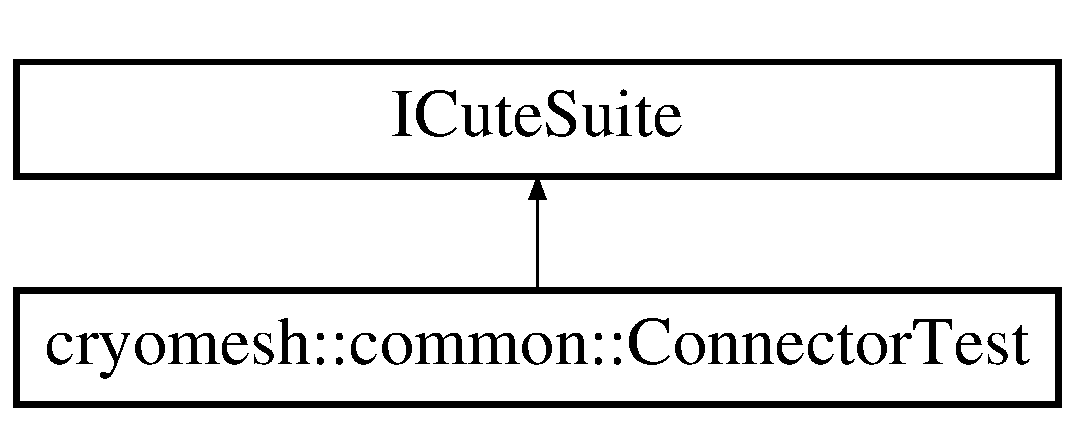
\includegraphics[height=2.000000cm]{classcryomesh_1_1common_1_1_connector_test}
\end{center}
\end{figure}
\subsection*{Public Member Functions}
\begin{DoxyCompactItemize}
\item 
\hyperlink{classcryomesh_1_1common_1_1_connector_test_a3b7373410094dd3dcb6f9779b4bedb22}{ConnectorTest} ()
\item 
virtual \hyperlink{classcryomesh_1_1common_1_1_connector_test_acf3e82456fe46ad459b986684d3f91f5}{$\sim$ConnectorTest} ()
\end{DoxyCompactItemize}
\subsection*{Static Public Member Functions}
\begin{DoxyCompactItemize}
\item 
static void \hyperlink{classcryomesh_1_1common_1_1_connector_test_a29e3a5baf1934101fa97e27e59f78631}{runSuite} ()
\item 
static void \hyperlink{classcryomesh_1_1common_1_1_connector_test_a710121de59188067a7da827bd98f8a9c}{testConnectDisconnect} ()
\end{DoxyCompactItemize}


\subsection{Constructor \& Destructor Documentation}
\hypertarget{classcryomesh_1_1common_1_1_connector_test_a3b7373410094dd3dcb6f9779b4bedb22}{
\index{cryomesh::common::ConnectorTest@{cryomesh::common::ConnectorTest}!ConnectorTest@{ConnectorTest}}
\index{ConnectorTest@{ConnectorTest}!cryomesh::common::ConnectorTest@{cryomesh::common::ConnectorTest}}
\subsubsection[{ConnectorTest}]{\setlength{\rightskip}{0pt plus 5cm}cryomesh::common::ConnectorTest::ConnectorTest (
\begin{DoxyParamCaption}
{}
\end{DoxyParamCaption}
)}}
\label{classcryomesh_1_1common_1_1_connector_test_a3b7373410094dd3dcb6f9779b4bedb22}
\hypertarget{classcryomesh_1_1common_1_1_connector_test_acf3e82456fe46ad459b986684d3f91f5}{
\index{cryomesh::common::ConnectorTest@{cryomesh::common::ConnectorTest}!$\sim$ConnectorTest@{$\sim$ConnectorTest}}
\index{$\sim$ConnectorTest@{$\sim$ConnectorTest}!cryomesh::common::ConnectorTest@{cryomesh::common::ConnectorTest}}
\subsubsection[{$\sim$ConnectorTest}]{\setlength{\rightskip}{0pt plus 5cm}cryomesh::common::ConnectorTest::$\sim$ConnectorTest (
\begin{DoxyParamCaption}
{}
\end{DoxyParamCaption}
)\hspace{0.3cm}{\ttfamily  \mbox{[}virtual\mbox{]}}}}
\label{classcryomesh_1_1common_1_1_connector_test_acf3e82456fe46ad459b986684d3f91f5}


\subsection{Member Function Documentation}
\hypertarget{classcryomesh_1_1common_1_1_connector_test_a29e3a5baf1934101fa97e27e59f78631}{
\index{cryomesh::common::ConnectorTest@{cryomesh::common::ConnectorTest}!runSuite@{runSuite}}
\index{runSuite@{runSuite}!cryomesh::common::ConnectorTest@{cryomesh::common::ConnectorTest}}
\subsubsection[{runSuite}]{\setlength{\rightskip}{0pt plus 5cm}void cryomesh::common::ConnectorTest::runSuite (
\begin{DoxyParamCaption}
{}
\end{DoxyParamCaption}
)\hspace{0.3cm}{\ttfamily  \mbox{[}static\mbox{]}}}}
\label{classcryomesh_1_1common_1_1_connector_test_a29e3a5baf1934101fa97e27e59f78631}
\hypertarget{classcryomesh_1_1common_1_1_connector_test_a710121de59188067a7da827bd98f8a9c}{
\index{cryomesh::common::ConnectorTest@{cryomesh::common::ConnectorTest}!testConnectDisconnect@{testConnectDisconnect}}
\index{testConnectDisconnect@{testConnectDisconnect}!cryomesh::common::ConnectorTest@{cryomesh::common::ConnectorTest}}
\subsubsection[{testConnectDisconnect}]{\setlength{\rightskip}{0pt plus 5cm}void cryomesh::common::ConnectorTest::testConnectDisconnect (
\begin{DoxyParamCaption}
{}
\end{DoxyParamCaption}
)\hspace{0.3cm}{\ttfamily  \mbox{[}static\mbox{]}}}}
\label{classcryomesh_1_1common_1_1_connector_test_a710121de59188067a7da827bd98f8a9c}


The documentation for this class was generated from the following files:\begin{DoxyCompactItemize}
\item 
src/common/\hyperlink{_connector_test_8h}{ConnectorTest.h}\item 
src/common/\hyperlink{_connector_test_8cpp}{ConnectorTest.cpp}\end{DoxyCompactItemize}

\hypertarget{classcryomesh_1_1common_1_1_containers_test}{
\section{cryomesh::common::ContainersTest Class Reference}
\label{classcryomesh_1_1common_1_1_containers_test}\index{cryomesh::common::ContainersTest@{cryomesh::common::ContainersTest}}
}


{\ttfamily \#include $<$ContainersTest.h$>$}

\subsection*{Public Member Functions}
\begin{DoxyCompactItemize}
\item 
virtual \hyperlink{classcryomesh_1_1common_1_1_containers_test_adb6d3d320b5815119a715b3fd84b85dc}{$\sim$ContainersTest} ()
\end{DoxyCompactItemize}
\subsection*{Static Public Member Functions}
\begin{DoxyCompactItemize}
\item 
static void \hyperlink{classcryomesh_1_1common_1_1_containers_test_aaa3fdced3fbec0ee448776d1c3923b7c}{runSuite} ()
\item 
static void \hyperlink{classcryomesh_1_1common_1_1_containers_test_a01358396840aa1cdb811aa0412caea47}{testCompare} ()
\item 
static void \hyperlink{classcryomesh_1_1common_1_1_containers_test_a36e9b84b40110b9f9ba37cc2ac5b4cd6}{testAdd} ()
\end{DoxyCompactItemize}
\subsection*{Protected Member Functions}
\begin{DoxyCompactItemize}
\item 
\hyperlink{classcryomesh_1_1common_1_1_containers_test_ae57f1e70d5904be4353ec3deec4d2bbf}{ContainersTest} ()
\end{DoxyCompactItemize}


\subsection{Constructor \& Destructor Documentation}
\hypertarget{classcryomesh_1_1common_1_1_containers_test_adb6d3d320b5815119a715b3fd84b85dc}{
\index{cryomesh::common::ContainersTest@{cryomesh::common::ContainersTest}!$\sim$ContainersTest@{$\sim$ContainersTest}}
\index{$\sim$ContainersTest@{$\sim$ContainersTest}!cryomesh::common::ContainersTest@{cryomesh::common::ContainersTest}}
\subsubsection[{$\sim$ContainersTest}]{\setlength{\rightskip}{0pt plus 5cm}virtual cryomesh::common::ContainersTest::$\sim$ContainersTest (
\begin{DoxyParamCaption}
{}
\end{DoxyParamCaption}
)\hspace{0.3cm}{\ttfamily  \mbox{[}inline, virtual\mbox{]}}}}
\label{classcryomesh_1_1common_1_1_containers_test_adb6d3d320b5815119a715b3fd84b85dc}
\hypertarget{classcryomesh_1_1common_1_1_containers_test_ae57f1e70d5904be4353ec3deec4d2bbf}{
\index{cryomesh::common::ContainersTest@{cryomesh::common::ContainersTest}!ContainersTest@{ContainersTest}}
\index{ContainersTest@{ContainersTest}!cryomesh::common::ContainersTest@{cryomesh::common::ContainersTest}}
\subsubsection[{ContainersTest}]{\setlength{\rightskip}{0pt plus 5cm}cryomesh::common::ContainersTest::ContainersTest (
\begin{DoxyParamCaption}
{}
\end{DoxyParamCaption}
)\hspace{0.3cm}{\ttfamily  \mbox{[}inline, protected\mbox{]}}}}
\label{classcryomesh_1_1common_1_1_containers_test_ae57f1e70d5904be4353ec3deec4d2bbf}


\subsection{Member Function Documentation}
\hypertarget{classcryomesh_1_1common_1_1_containers_test_aaa3fdced3fbec0ee448776d1c3923b7c}{
\index{cryomesh::common::ContainersTest@{cryomesh::common::ContainersTest}!runSuite@{runSuite}}
\index{runSuite@{runSuite}!cryomesh::common::ContainersTest@{cryomesh::common::ContainersTest}}
\subsubsection[{runSuite}]{\setlength{\rightskip}{0pt plus 5cm}void cryomesh::common::ContainersTest::runSuite (
\begin{DoxyParamCaption}
{}
\end{DoxyParamCaption}
)\hspace{0.3cm}{\ttfamily  \mbox{[}static\mbox{]}}}}
\label{classcryomesh_1_1common_1_1_containers_test_aaa3fdced3fbec0ee448776d1c3923b7c}
\hypertarget{classcryomesh_1_1common_1_1_containers_test_a36e9b84b40110b9f9ba37cc2ac5b4cd6}{
\index{cryomesh::common::ContainersTest@{cryomesh::common::ContainersTest}!testAdd@{testAdd}}
\index{testAdd@{testAdd}!cryomesh::common::ContainersTest@{cryomesh::common::ContainersTest}}
\subsubsection[{testAdd}]{\setlength{\rightskip}{0pt plus 5cm}void cryomesh::common::ContainersTest::testAdd (
\begin{DoxyParamCaption}
{}
\end{DoxyParamCaption}
)\hspace{0.3cm}{\ttfamily  \mbox{[}static\mbox{]}}}}
\label{classcryomesh_1_1common_1_1_containers_test_a36e9b84b40110b9f9ba37cc2ac5b4cd6}
\hypertarget{classcryomesh_1_1common_1_1_containers_test_a01358396840aa1cdb811aa0412caea47}{
\index{cryomesh::common::ContainersTest@{cryomesh::common::ContainersTest}!testCompare@{testCompare}}
\index{testCompare@{testCompare}!cryomesh::common::ContainersTest@{cryomesh::common::ContainersTest}}
\subsubsection[{testCompare}]{\setlength{\rightskip}{0pt plus 5cm}void cryomesh::common::ContainersTest::testCompare (
\begin{DoxyParamCaption}
{}
\end{DoxyParamCaption}
)\hspace{0.3cm}{\ttfamily  \mbox{[}static\mbox{]}}}}
\label{classcryomesh_1_1common_1_1_containers_test_a01358396840aa1cdb811aa0412caea47}


The documentation for this class was generated from the following files:\begin{DoxyCompactItemize}
\item 
src/common/\hyperlink{_containers_test_8h}{ContainersTest.h}\item 
src/common/\hyperlink{_containers_test_8cpp}{ContainersTest.cpp}\end{DoxyCompactItemize}

\hypertarget{class_core_tests_defaults}{
\section{CoreTestsDefaults Class Reference}
\label{class_core_tests_defaults}\index{CoreTestsDefaults@{CoreTestsDefaults}}
}


{\ttfamily \#include $<$CoreTestsDefaults.h$>$}

\subsection*{Public Member Functions}
\begin{DoxyCompactItemize}
\item 
virtual \hyperlink{class_core_tests_defaults_a34f48ea5b64f852fdd44ac4d378df6e8}{$\sim$CoreTestsDefaults} ()
\end{DoxyCompactItemize}
\subsection*{Static Public Attributes}
\begin{DoxyCompactItemize}
\item 
static const std::string \hyperlink{class_core_tests_defaults_aa543f63f7c94e1f66868b318c72f4b59}{TEST\_\-DIRECTORY} = \char`\"{}TestData/Tests/\char`\"{}
\end{DoxyCompactItemize}
\subsection*{Private Member Functions}
\begin{DoxyCompactItemize}
\item 
\hyperlink{class_core_tests_defaults_a861acd8b537c1880c86b9a00e4ec5100}{CoreTestsDefaults} ()
\end{DoxyCompactItemize}


\subsection{Constructor \& Destructor Documentation}
\hypertarget{class_core_tests_defaults_a34f48ea5b64f852fdd44ac4d378df6e8}{
\index{CoreTestsDefaults@{CoreTestsDefaults}!$\sim$CoreTestsDefaults@{$\sim$CoreTestsDefaults}}
\index{$\sim$CoreTestsDefaults@{$\sim$CoreTestsDefaults}!CoreTestsDefaults@{CoreTestsDefaults}}
\subsubsection[{$\sim$CoreTestsDefaults}]{\setlength{\rightskip}{0pt plus 5cm}CoreTestsDefaults::$\sim$CoreTestsDefaults (
\begin{DoxyParamCaption}
{}
\end{DoxyParamCaption}
)\hspace{0.3cm}{\ttfamily  \mbox{[}virtual\mbox{]}}}}
\label{class_core_tests_defaults_a34f48ea5b64f852fdd44ac4d378df6e8}
\hypertarget{class_core_tests_defaults_a861acd8b537c1880c86b9a00e4ec5100}{
\index{CoreTestsDefaults@{CoreTestsDefaults}!CoreTestsDefaults@{CoreTestsDefaults}}
\index{CoreTestsDefaults@{CoreTestsDefaults}!CoreTestsDefaults@{CoreTestsDefaults}}
\subsubsection[{CoreTestsDefaults}]{\setlength{\rightskip}{0pt plus 5cm}CoreTestsDefaults::CoreTestsDefaults (
\begin{DoxyParamCaption}
{}
\end{DoxyParamCaption}
)\hspace{0.3cm}{\ttfamily  \mbox{[}private\mbox{]}}}}
\label{class_core_tests_defaults_a861acd8b537c1880c86b9a00e4ec5100}


\subsection{Member Data Documentation}
\hypertarget{class_core_tests_defaults_aa543f63f7c94e1f66868b318c72f4b59}{
\index{CoreTestsDefaults@{CoreTestsDefaults}!TEST\_\-DIRECTORY@{TEST\_\-DIRECTORY}}
\index{TEST\_\-DIRECTORY@{TEST\_\-DIRECTORY}!CoreTestsDefaults@{CoreTestsDefaults}}
\subsubsection[{TEST\_\-DIRECTORY}]{\setlength{\rightskip}{0pt plus 5cm}const std::string {\bf CoreTestsDefaults::TEST\_\-DIRECTORY} = \char`\"{}TestData/Tests/\char`\"{}\hspace{0.3cm}{\ttfamily  \mbox{[}static\mbox{]}}}}
\label{class_core_tests_defaults_aa543f63f7c94e1f66868b318c72f4b59}


The documentation for this class was generated from the following files:\begin{DoxyCompactItemize}
\item 
src/\hyperlink{_core_tests_defaults_8h}{CoreTestsDefaults.h}\item 
src/\hyperlink{_core_tests_defaults_8cpp}{CoreTestsDefaults.cpp}\end{DoxyCompactItemize}

\hypertarget{class_i_cute_suite}{
\section{ICuteSuite Class Reference}
\label{class_i_cute_suite}\index{ICuteSuite@{ICuteSuite}}
}


{\ttfamily \#include $<$ICuteSuite.h$>$}

Inheritance diagram for ICuteSuite:\begin{figure}[H]
\begin{center}
\leavevmode
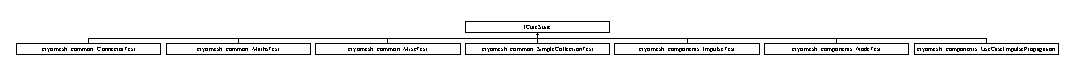
\includegraphics[height=0.509554cm]{class_i_cute_suite}
\end{center}
\end{figure}
\subsection*{Public Member Functions}
\begin{DoxyCompactItemize}
\item 
virtual \hyperlink{class_i_cute_suite_a34d5fdc00c00dff25c385d0ff31032c9}{$\sim$ICuteSuite} ()
\end{DoxyCompactItemize}


\subsection{Constructor \& Destructor Documentation}
\hypertarget{class_i_cute_suite_a34d5fdc00c00dff25c385d0ff31032c9}{
\index{ICuteSuite@{ICuteSuite}!$\sim$ICuteSuite@{$\sim$ICuteSuite}}
\index{$\sim$ICuteSuite@{$\sim$ICuteSuite}!ICuteSuite@{ICuteSuite}}
\subsubsection[{$\sim$ICuteSuite}]{\setlength{\rightskip}{0pt plus 5cm}virtual ICuteSuite::$\sim$ICuteSuite (
\begin{DoxyParamCaption}
{}
\end{DoxyParamCaption}
)\hspace{0.3cm}{\ttfamily  \mbox{[}inline, virtual\mbox{]}}}}
\label{class_i_cute_suite_a34d5fdc00c00dff25c385d0ff31032c9}


The documentation for this class was generated from the following file:\begin{DoxyCompactItemize}
\item 
src/\hyperlink{_i_cute_suite_8h}{ICuteSuite.h}\end{DoxyCompactItemize}

\hypertarget{classcryomesh_1_1components_1_1_impulse_collection_test}{
\section{cryomesh::components::ImpulseCollectionTest Class Reference}
\label{classcryomesh_1_1components_1_1_impulse_collection_test}\index{cryomesh::components::ImpulseCollectionTest@{cryomesh::components::ImpulseCollectionTest}}
}


{\ttfamily \#include $<$ImpulseCollectionTest.h$>$}

\subsection*{Static Public Member Functions}
\begin{DoxyCompactItemize}
\item 
static void \hyperlink{classcryomesh_1_1components_1_1_impulse_collection_test_a5f1a65b6809e590a5f61fdac8270980f}{runSuite} ()
\item 
static void \hyperlink{classcryomesh_1_1components_1_1_impulse_collection_test_abf43f9a14bc655307ea996a3165914fe}{testAddRemoveImpulses} ()
\item 
static void \hyperlink{classcryomesh_1_1components_1_1_impulse_collection_test_ac4495af7ab2857295d14b479ee86ab2a}{testClear} ()
\item 
static void \hyperlink{classcryomesh_1_1components_1_1_impulse_collection_test_a39f5cdc7c00668f772230e80264215cb}{testGetActivity} ()
\item 
static void \hyperlink{classcryomesh_1_1components_1_1_impulse_collection_test_aa48e2413cef48b15c58b6e2f05480fc9}{testOperators} ()
\end{DoxyCompactItemize}


\subsection{Detailed Description}
Collection of tests for ImpulseCollection 

\subsection{Member Function Documentation}
\hypertarget{classcryomesh_1_1components_1_1_impulse_collection_test_a5f1a65b6809e590a5f61fdac8270980f}{
\index{cryomesh::components::ImpulseCollectionTest@{cryomesh::components::ImpulseCollectionTest}!runSuite@{runSuite}}
\index{runSuite@{runSuite}!cryomesh::components::ImpulseCollectionTest@{cryomesh::components::ImpulseCollectionTest}}
\subsubsection[{runSuite}]{\setlength{\rightskip}{0pt plus 5cm}void cryomesh::components::ImpulseCollectionTest::runSuite (
\begin{DoxyParamCaption}
{}
\end{DoxyParamCaption}
)\hspace{0.3cm}{\ttfamily  \mbox{[}static\mbox{]}}}}
\label{classcryomesh_1_1components_1_1_impulse_collection_test_a5f1a65b6809e590a5f61fdac8270980f}
Run all tests \hypertarget{classcryomesh_1_1components_1_1_impulse_collection_test_abf43f9a14bc655307ea996a3165914fe}{
\index{cryomesh::components::ImpulseCollectionTest@{cryomesh::components::ImpulseCollectionTest}!testAddRemoveImpulses@{testAddRemoveImpulses}}
\index{testAddRemoveImpulses@{testAddRemoveImpulses}!cryomesh::components::ImpulseCollectionTest@{cryomesh::components::ImpulseCollectionTest}}
\subsubsection[{testAddRemoveImpulses}]{\setlength{\rightskip}{0pt plus 5cm}void cryomesh::components::ImpulseCollectionTest::testAddRemoveImpulses (
\begin{DoxyParamCaption}
{}
\end{DoxyParamCaption}
)\hspace{0.3cm}{\ttfamily  \mbox{[}static\mbox{]}}}}
\label{classcryomesh_1_1components_1_1_impulse_collection_test_abf43f9a14bc655307ea996a3165914fe}
Test adding and removing impulses \hypertarget{classcryomesh_1_1components_1_1_impulse_collection_test_ac4495af7ab2857295d14b479ee86ab2a}{
\index{cryomesh::components::ImpulseCollectionTest@{cryomesh::components::ImpulseCollectionTest}!testClear@{testClear}}
\index{testClear@{testClear}!cryomesh::components::ImpulseCollectionTest@{cryomesh::components::ImpulseCollectionTest}}
\subsubsection[{testClear}]{\setlength{\rightskip}{0pt plus 5cm}void cryomesh::components::ImpulseCollectionTest::testClear (
\begin{DoxyParamCaption}
{}
\end{DoxyParamCaption}
)\hspace{0.3cm}{\ttfamily  \mbox{[}static\mbox{]}}}}
\label{classcryomesh_1_1components_1_1_impulse_collection_test_ac4495af7ab2857295d14b479ee86ab2a}
Test clearing functions \hypertarget{classcryomesh_1_1components_1_1_impulse_collection_test_a39f5cdc7c00668f772230e80264215cb}{
\index{cryomesh::components::ImpulseCollectionTest@{cryomesh::components::ImpulseCollectionTest}!testGetActivity@{testGetActivity}}
\index{testGetActivity@{testGetActivity}!cryomesh::components::ImpulseCollectionTest@{cryomesh::components::ImpulseCollectionTest}}
\subsubsection[{testGetActivity}]{\setlength{\rightskip}{0pt plus 5cm}void cryomesh::components::ImpulseCollectionTest::testGetActivity (
\begin{DoxyParamCaption}
{}
\end{DoxyParamCaption}
)\hspace{0.3cm}{\ttfamily  \mbox{[}static\mbox{]}}}}
\label{classcryomesh_1_1components_1_1_impulse_collection_test_a39f5cdc7c00668f772230e80264215cb}
Test activity calculation \hypertarget{classcryomesh_1_1components_1_1_impulse_collection_test_aa48e2413cef48b15c58b6e2f05480fc9}{
\index{cryomesh::components::ImpulseCollectionTest@{cryomesh::components::ImpulseCollectionTest}!testOperators@{testOperators}}
\index{testOperators@{testOperators}!cryomesh::components::ImpulseCollectionTest@{cryomesh::components::ImpulseCollectionTest}}
\subsubsection[{testOperators}]{\setlength{\rightskip}{0pt plus 5cm}void cryomesh::components::ImpulseCollectionTest::testOperators (
\begin{DoxyParamCaption}
{}
\end{DoxyParamCaption}
)\hspace{0.3cm}{\ttfamily  \mbox{[}static\mbox{]}}}}
\label{classcryomesh_1_1components_1_1_impulse_collection_test_aa48e2413cef48b15c58b6e2f05480fc9}
Test operators 

The documentation for this class was generated from the following files:\begin{DoxyCompactItemize}
\item 
src/components/\hyperlink{_impulse_collection_test_8h}{ImpulseCollectionTest.h}\item 
src/components/\hyperlink{_impulse_collection_test_8cpp}{ImpulseCollectionTest.cpp}\end{DoxyCompactItemize}

\hypertarget{classcryomesh_1_1components_1_1_impulse_test}{
\section{cryomesh::components::ImpulseTest Class Reference}
\label{classcryomesh_1_1components_1_1_impulse_test}\index{cryomesh::components::ImpulseTest@{cryomesh::components::ImpulseTest}}
}


{\ttfamily \#include $<$ImpulseTest.h$>$}

Inheritance diagram for cryomesh::components::ImpulseTest:\begin{figure}[H]
\begin{center}
\leavevmode
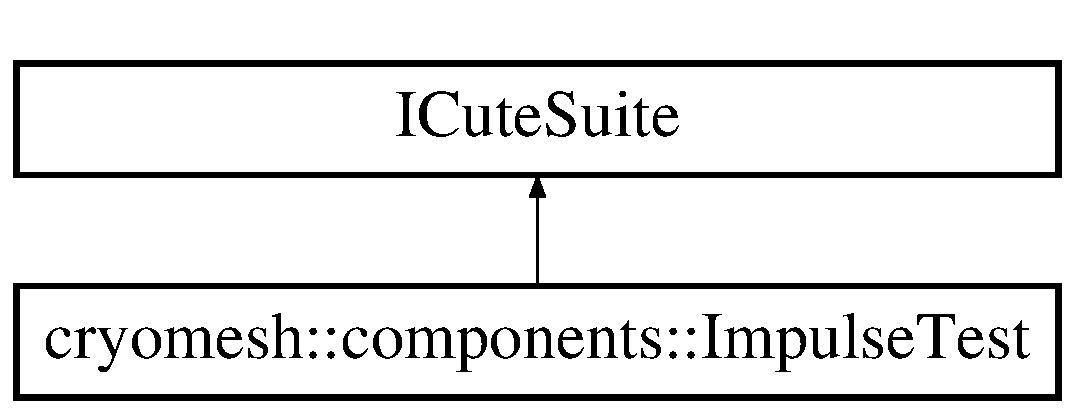
\includegraphics[height=2.000000cm]{classcryomesh_1_1components_1_1_impulse_test}
\end{center}
\end{figure}
\subsection*{Public Member Functions}
\begin{DoxyCompactItemize}
\item 
\hyperlink{classcryomesh_1_1components_1_1_impulse_test_adcf8973dc76591a1fdf27dee6e9c18e1}{ImpulseTest} ()
\item 
virtual \hyperlink{classcryomesh_1_1components_1_1_impulse_test_af6e2a24a4795115f5fa205612845fd61}{$\sim$ImpulseTest} ()
\end{DoxyCompactItemize}
\subsection*{Static Public Member Functions}
\begin{DoxyCompactItemize}
\item 
static void \hyperlink{classcryomesh_1_1components_1_1_impulse_test_a3650059bffacf3cc31c840e00a77f80e}{runSuite} ()
\item 
static void \hyperlink{classcryomesh_1_1components_1_1_impulse_test_a048013cfdeba94c1587fcbc8e992ec70}{testActivityCreation} ()
\item 
static void \hyperlink{classcryomesh_1_1components_1_1_impulse_test_ab67967fa81e21598294119f8e0095481}{testActivityMaxMin} ()
\item 
static void \hyperlink{classcryomesh_1_1components_1_1_impulse_test_a4ccfa7131ff634e9da8b42d9a1ce1206}{testActiveCycles} ()
\item 
static void \hyperlink{classcryomesh_1_1components_1_1_impulse_test_a8c6afd6637b1fadedf6986c6ddb60b38}{testOperators} ()
\end{DoxyCompactItemize}


\subsection{Constructor \& Destructor Documentation}
\hypertarget{classcryomesh_1_1components_1_1_impulse_test_adcf8973dc76591a1fdf27dee6e9c18e1}{
\index{cryomesh::components::ImpulseTest@{cryomesh::components::ImpulseTest}!ImpulseTest@{ImpulseTest}}
\index{ImpulseTest@{ImpulseTest}!cryomesh::components::ImpulseTest@{cryomesh::components::ImpulseTest}}
\subsubsection[{ImpulseTest}]{\setlength{\rightskip}{0pt plus 5cm}cryomesh::components::ImpulseTest::ImpulseTest (
\begin{DoxyParamCaption}
{}
\end{DoxyParamCaption}
)}}
\label{classcryomesh_1_1components_1_1_impulse_test_adcf8973dc76591a1fdf27dee6e9c18e1}
\hypertarget{classcryomesh_1_1components_1_1_impulse_test_af6e2a24a4795115f5fa205612845fd61}{
\index{cryomesh::components::ImpulseTest@{cryomesh::components::ImpulseTest}!$\sim$ImpulseTest@{$\sim$ImpulseTest}}
\index{$\sim$ImpulseTest@{$\sim$ImpulseTest}!cryomesh::components::ImpulseTest@{cryomesh::components::ImpulseTest}}
\subsubsection[{$\sim$ImpulseTest}]{\setlength{\rightskip}{0pt plus 5cm}cryomesh::components::ImpulseTest::$\sim$ImpulseTest (
\begin{DoxyParamCaption}
{}
\end{DoxyParamCaption}
)\hspace{0.3cm}{\ttfamily  \mbox{[}virtual\mbox{]}}}}
\label{classcryomesh_1_1components_1_1_impulse_test_af6e2a24a4795115f5fa205612845fd61}


\subsection{Member Function Documentation}
\hypertarget{classcryomesh_1_1components_1_1_impulse_test_a3650059bffacf3cc31c840e00a77f80e}{
\index{cryomesh::components::ImpulseTest@{cryomesh::components::ImpulseTest}!runSuite@{runSuite}}
\index{runSuite@{runSuite}!cryomesh::components::ImpulseTest@{cryomesh::components::ImpulseTest}}
\subsubsection[{runSuite}]{\setlength{\rightskip}{0pt plus 5cm}void cryomesh::components::ImpulseTest::runSuite (
\begin{DoxyParamCaption}
{}
\end{DoxyParamCaption}
)\hspace{0.3cm}{\ttfamily  \mbox{[}static\mbox{]}}}}
\label{classcryomesh_1_1components_1_1_impulse_test_a3650059bffacf3cc31c840e00a77f80e}
Run all tests \hypertarget{classcryomesh_1_1components_1_1_impulse_test_a4ccfa7131ff634e9da8b42d9a1ce1206}{
\index{cryomesh::components::ImpulseTest@{cryomesh::components::ImpulseTest}!testActiveCycles@{testActiveCycles}}
\index{testActiveCycles@{testActiveCycles}!cryomesh::components::ImpulseTest@{cryomesh::components::ImpulseTest}}
\subsubsection[{testActiveCycles}]{\setlength{\rightskip}{0pt plus 5cm}void cryomesh::components::ImpulseTest::testActiveCycles (
\begin{DoxyParamCaption}
{}
\end{DoxyParamCaption}
)\hspace{0.3cm}{\ttfamily  \mbox{[}static\mbox{]}}}}
\label{classcryomesh_1_1components_1_1_impulse_test_a4ccfa7131ff634e9da8b42d9a1ce1206}
Test working with active cycles \hypertarget{classcryomesh_1_1components_1_1_impulse_test_a048013cfdeba94c1587fcbc8e992ec70}{
\index{cryomesh::components::ImpulseTest@{cryomesh::components::ImpulseTest}!testActivityCreation@{testActivityCreation}}
\index{testActivityCreation@{testActivityCreation}!cryomesh::components::ImpulseTest@{cryomesh::components::ImpulseTest}}
\subsubsection[{testActivityCreation}]{\setlength{\rightskip}{0pt plus 5cm}void cryomesh::components::ImpulseTest::testActivityCreation (
\begin{DoxyParamCaption}
{}
\end{DoxyParamCaption}
)\hspace{0.3cm}{\ttfamily  \mbox{[}static\mbox{]}}}}
\label{classcryomesh_1_1components_1_1_impulse_test_a048013cfdeba94c1587fcbc8e992ec70}
Test the creation of activity graphs \hypertarget{classcryomesh_1_1components_1_1_impulse_test_ab67967fa81e21598294119f8e0095481}{
\index{cryomesh::components::ImpulseTest@{cryomesh::components::ImpulseTest}!testActivityMaxMin@{testActivityMaxMin}}
\index{testActivityMaxMin@{testActivityMaxMin}!cryomesh::components::ImpulseTest@{cryomesh::components::ImpulseTest}}
\subsubsection[{testActivityMaxMin}]{\setlength{\rightskip}{0pt plus 5cm}void cryomesh::components::ImpulseTest::testActivityMaxMin (
\begin{DoxyParamCaption}
{}
\end{DoxyParamCaption}
)\hspace{0.3cm}{\ttfamily  \mbox{[}static\mbox{]}}}}
\label{classcryomesh_1_1components_1_1_impulse_test_ab67967fa81e21598294119f8e0095481}
Test getting activity max and mins \hypertarget{classcryomesh_1_1components_1_1_impulse_test_a8c6afd6637b1fadedf6986c6ddb60b38}{
\index{cryomesh::components::ImpulseTest@{cryomesh::components::ImpulseTest}!testOperators@{testOperators}}
\index{testOperators@{testOperators}!cryomesh::components::ImpulseTest@{cryomesh::components::ImpulseTest}}
\subsubsection[{testOperators}]{\setlength{\rightskip}{0pt plus 5cm}void cryomesh::components::ImpulseTest::testOperators (
\begin{DoxyParamCaption}
{}
\end{DoxyParamCaption}
)\hspace{0.3cm}{\ttfamily  \mbox{[}static\mbox{]}}}}
\label{classcryomesh_1_1components_1_1_impulse_test_a8c6afd6637b1fadedf6986c6ddb60b38}
Test all operators 

The documentation for this class was generated from the following files:\begin{DoxyCompactItemize}
\item 
src/components/\hyperlink{_impulse_test_8h}{ImpulseTest.h}\item 
src/components/\hyperlink{_impulse_test_8cpp}{ImpulseTest.cpp}\end{DoxyCompactItemize}

\hypertarget{classcryomesh_1_1common_1_1_maths_test}{
\section{cryomesh::common::MathsTest Class Reference}
\label{classcryomesh_1_1common_1_1_maths_test}\index{cryomesh::common::MathsTest@{cryomesh::common::MathsTest}}
}


{\ttfamily \#include $<$MathsTest.h$>$}

Inheritance diagram for cryomesh::common::MathsTest:\begin{figure}[H]
\begin{center}
\leavevmode
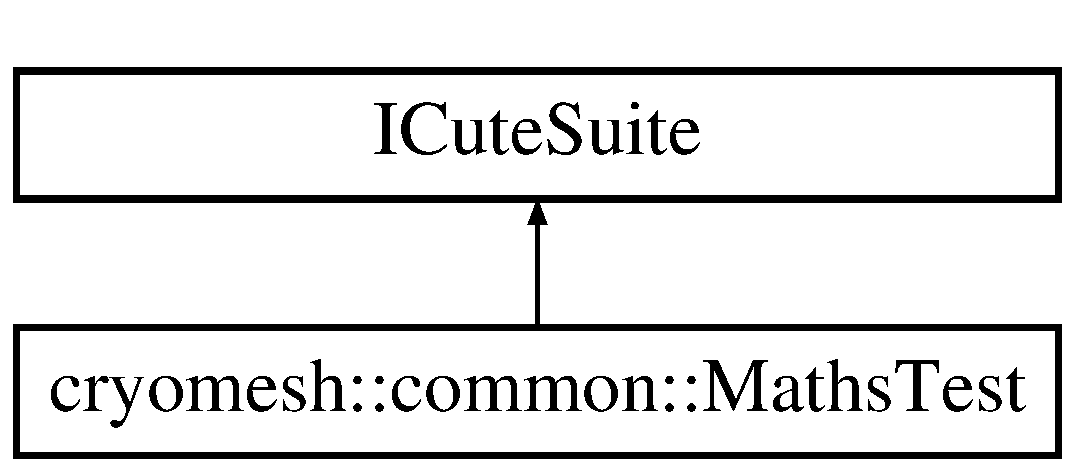
\includegraphics[height=2.000000cm]{classcryomesh_1_1common_1_1_maths_test}
\end{center}
\end{figure}
\subsection*{Public Member Functions}
\begin{DoxyCompactItemize}
\item 
\hyperlink{classcryomesh_1_1common_1_1_maths_test_a23f4e79814ad2077c29e505d03e1a066}{MathsTest} ()
\item 
virtual \hyperlink{classcryomesh_1_1common_1_1_maths_test_a2fbabfe02cbf4be738cdf14448039834}{$\sim$MathsTest} ()
\end{DoxyCompactItemize}
\subsection*{Static Public Member Functions}
\begin{DoxyCompactItemize}
\item 
static void \hyperlink{classcryomesh_1_1common_1_1_maths_test_ac8ff61d96b4026c9eed348d851b6b4fa}{runSuite} ()
\item 
static void \hyperlink{classcryomesh_1_1common_1_1_maths_test_acd403b741ca1c9ad580b8dfafd097ca2}{testGetRandomValue} ()
\end{DoxyCompactItemize}


\subsection{Constructor \& Destructor Documentation}
\hypertarget{classcryomesh_1_1common_1_1_maths_test_a23f4e79814ad2077c29e505d03e1a066}{
\index{cryomesh::common::MathsTest@{cryomesh::common::MathsTest}!MathsTest@{MathsTest}}
\index{MathsTest@{MathsTest}!cryomesh::common::MathsTest@{cryomesh::common::MathsTest}}
\subsubsection[{MathsTest}]{\setlength{\rightskip}{0pt plus 5cm}cryomesh::common::MathsTest::MathsTest (
\begin{DoxyParamCaption}
{}
\end{DoxyParamCaption}
)}}
\label{classcryomesh_1_1common_1_1_maths_test_a23f4e79814ad2077c29e505d03e1a066}
\hypertarget{classcryomesh_1_1common_1_1_maths_test_a2fbabfe02cbf4be738cdf14448039834}{
\index{cryomesh::common::MathsTest@{cryomesh::common::MathsTest}!$\sim$MathsTest@{$\sim$MathsTest}}
\index{$\sim$MathsTest@{$\sim$MathsTest}!cryomesh::common::MathsTest@{cryomesh::common::MathsTest}}
\subsubsection[{$\sim$MathsTest}]{\setlength{\rightskip}{0pt plus 5cm}cryomesh::common::MathsTest::$\sim$MathsTest (
\begin{DoxyParamCaption}
{}
\end{DoxyParamCaption}
)\hspace{0.3cm}{\ttfamily  \mbox{[}virtual\mbox{]}}}}
\label{classcryomesh_1_1common_1_1_maths_test_a2fbabfe02cbf4be738cdf14448039834}


\subsection{Member Function Documentation}
\hypertarget{classcryomesh_1_1common_1_1_maths_test_ac8ff61d96b4026c9eed348d851b6b4fa}{
\index{cryomesh::common::MathsTest@{cryomesh::common::MathsTest}!runSuite@{runSuite}}
\index{runSuite@{runSuite}!cryomesh::common::MathsTest@{cryomesh::common::MathsTest}}
\subsubsection[{runSuite}]{\setlength{\rightskip}{0pt plus 5cm}void cryomesh::common::MathsTest::runSuite (
\begin{DoxyParamCaption}
{}
\end{DoxyParamCaption}
)\hspace{0.3cm}{\ttfamily  \mbox{[}static\mbox{]}}}}
\label{classcryomesh_1_1common_1_1_maths_test_ac8ff61d96b4026c9eed348d851b6b4fa}
\hypertarget{classcryomesh_1_1common_1_1_maths_test_acd403b741ca1c9ad580b8dfafd097ca2}{
\index{cryomesh::common::MathsTest@{cryomesh::common::MathsTest}!testGetRandomValue@{testGetRandomValue}}
\index{testGetRandomValue@{testGetRandomValue}!cryomesh::common::MathsTest@{cryomesh::common::MathsTest}}
\subsubsection[{testGetRandomValue}]{\setlength{\rightskip}{0pt plus 5cm}void cryomesh::common::MathsTest::testGetRandomValue (
\begin{DoxyParamCaption}
{}
\end{DoxyParamCaption}
)\hspace{0.3cm}{\ttfamily  \mbox{[}static\mbox{]}}}}
\label{classcryomesh_1_1common_1_1_maths_test_acd403b741ca1c9ad580b8dfafd097ca2}


The documentation for this class was generated from the following files:\begin{DoxyCompactItemize}
\item 
src/common/\hyperlink{_maths_test_8h}{MathsTest.h}\item 
src/common/\hyperlink{_maths_test_8cpp}{MathsTest.cpp}\end{DoxyCompactItemize}

\hypertarget{classcryomesh_1_1common_1_1_misc_test}{
\section{cryomesh::common::MiscTest Class Reference}
\label{classcryomesh_1_1common_1_1_misc_test}\index{cryomesh::common::MiscTest@{cryomesh::common::MiscTest}}
}


{\ttfamily \#include $<$MiscTest.h$>$}

Inheritance diagram for cryomesh::common::MiscTest:\begin{figure}[H]
\begin{center}
\leavevmode
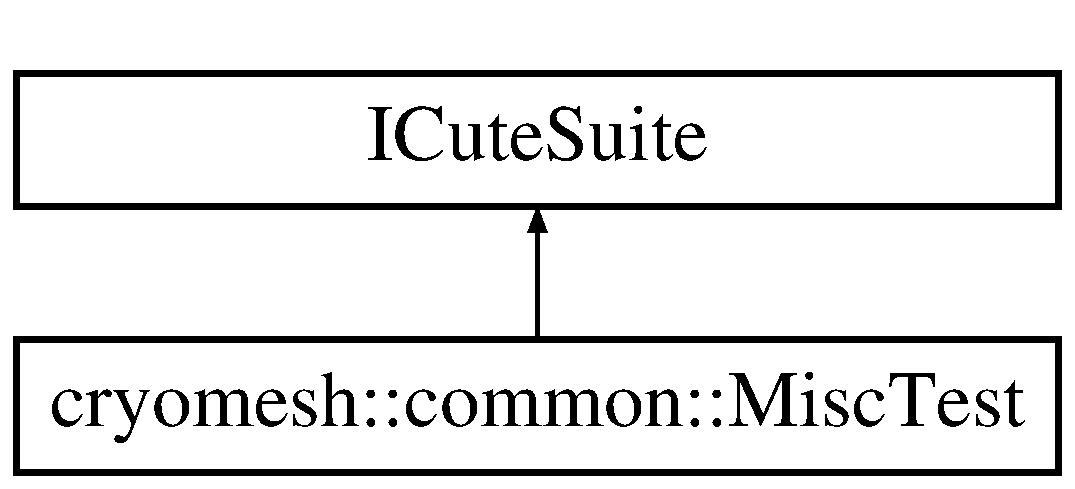
\includegraphics[height=2.000000cm]{classcryomesh_1_1common_1_1_misc_test}
\end{center}
\end{figure}
\subsection*{Static Public Member Functions}
\begin{DoxyCompactItemize}
\item 
static void \hyperlink{classcryomesh_1_1common_1_1_misc_test_acc5b0cd2668fa5ffd633a42e779f488d}{runSuite} ()
\item 
static void \hyperlink{classcryomesh_1_1common_1_1_misc_test_af2e14bca887d72af8846f558452612ea}{testparseArgs} ()
\item 
static void \hyperlink{classcryomesh_1_1common_1_1_misc_test_a89eb54f0a463bf2e331fde7eec992404}{testtoLower} ()
\item 
static void \hyperlink{classcryomesh_1_1common_1_1_misc_test_a9a69bbb484052a9d8cd57cd1c3ecef33}{testremoveChars} ()
\end{DoxyCompactItemize}


\subsection{Member Function Documentation}
\hypertarget{classcryomesh_1_1common_1_1_misc_test_acc5b0cd2668fa5ffd633a42e779f488d}{
\index{cryomesh::common::MiscTest@{cryomesh::common::MiscTest}!runSuite@{runSuite}}
\index{runSuite@{runSuite}!cryomesh::common::MiscTest@{cryomesh::common::MiscTest}}
\subsubsection[{runSuite}]{\setlength{\rightskip}{0pt plus 5cm}void cryomesh::common::MiscTest::runSuite (
\begin{DoxyParamCaption}
{}
\end{DoxyParamCaption}
)\hspace{0.3cm}{\ttfamily  \mbox{[}static\mbox{]}}}}
\label{classcryomesh_1_1common_1_1_misc_test_acc5b0cd2668fa5ffd633a42e779f488d}
\hypertarget{classcryomesh_1_1common_1_1_misc_test_af2e14bca887d72af8846f558452612ea}{
\index{cryomesh::common::MiscTest@{cryomesh::common::MiscTest}!testparseArgs@{testparseArgs}}
\index{testparseArgs@{testparseArgs}!cryomesh::common::MiscTest@{cryomesh::common::MiscTest}}
\subsubsection[{testparseArgs}]{\setlength{\rightskip}{0pt plus 5cm}void cryomesh::common::MiscTest::testparseArgs (
\begin{DoxyParamCaption}
{}
\end{DoxyParamCaption}
)\hspace{0.3cm}{\ttfamily  \mbox{[}static\mbox{]}}}}
\label{classcryomesh_1_1common_1_1_misc_test_af2e14bca887d72af8846f558452612ea}
\hypertarget{classcryomesh_1_1common_1_1_misc_test_a9a69bbb484052a9d8cd57cd1c3ecef33}{
\index{cryomesh::common::MiscTest@{cryomesh::common::MiscTest}!testremoveChars@{testremoveChars}}
\index{testremoveChars@{testremoveChars}!cryomesh::common::MiscTest@{cryomesh::common::MiscTest}}
\subsubsection[{testremoveChars}]{\setlength{\rightskip}{0pt plus 5cm}void cryomesh::common::MiscTest::testremoveChars (
\begin{DoxyParamCaption}
{}
\end{DoxyParamCaption}
)\hspace{0.3cm}{\ttfamily  \mbox{[}static\mbox{]}}}}
\label{classcryomesh_1_1common_1_1_misc_test_a9a69bbb484052a9d8cd57cd1c3ecef33}
\hypertarget{classcryomesh_1_1common_1_1_misc_test_a89eb54f0a463bf2e331fde7eec992404}{
\index{cryomesh::common::MiscTest@{cryomesh::common::MiscTest}!testtoLower@{testtoLower}}
\index{testtoLower@{testtoLower}!cryomesh::common::MiscTest@{cryomesh::common::MiscTest}}
\subsubsection[{testtoLower}]{\setlength{\rightskip}{0pt plus 5cm}void cryomesh::common::MiscTest::testtoLower (
\begin{DoxyParamCaption}
{}
\end{DoxyParamCaption}
)\hspace{0.3cm}{\ttfamily  \mbox{[}static\mbox{]}}}}
\label{classcryomesh_1_1common_1_1_misc_test_a89eb54f0a463bf2e331fde7eec992404}


The documentation for this class was generated from the following files:\begin{DoxyCompactItemize}
\item 
src/common/\hyperlink{_misc_test_8h}{MiscTest.h}\item 
src/common/\hyperlink{_misc_test_8cpp}{MiscTest.cpp}\end{DoxyCompactItemize}

\hypertarget{classcryomesh_1_1components_1_1_node_test}{
\section{cryomesh::components::NodeTest Class Reference}
\label{classcryomesh_1_1components_1_1_node_test}\index{cryomesh::components::NodeTest@{cryomesh::components::NodeTest}}
}


{\ttfamily \#include $<$NodeTest.h$>$}

Inheritance diagram for cryomesh::components::NodeTest:\begin{figure}[H]
\begin{center}
\leavevmode
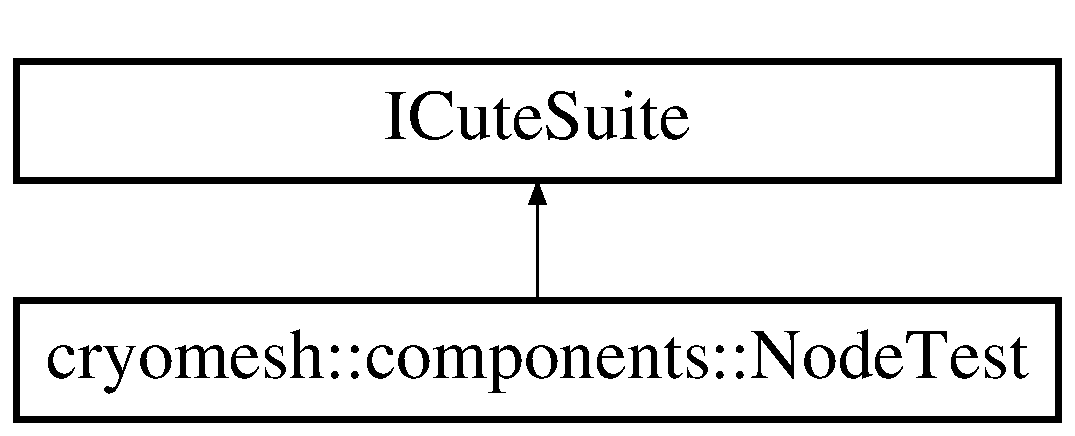
\includegraphics[height=2.000000cm]{classcryomesh_1_1components_1_1_node_test}
\end{center}
\end{figure}
\subsection*{Public Member Functions}
\begin{DoxyCompactItemize}
\item 
\hyperlink{classcryomesh_1_1components_1_1_node_test_ae8bb3c72288306e666d18696a5be7b35}{NodeTest} ()
\item 
virtual \hyperlink{classcryomesh_1_1components_1_1_node_test_a6a346d4f8e13c5aaa6b030b0587bcff9}{$\sim$NodeTest} ()
\end{DoxyCompactItemize}
\subsection*{Static Public Member Functions}
\begin{DoxyCompactItemize}
\item 
static void \hyperlink{classcryomesh_1_1components_1_1_node_test_a14815aa49eed66ddc12768b7a267fbf3}{runSuite} ()
\item 
static void \hyperlink{classcryomesh_1_1components_1_1_node_test_a79ace8c51f04945a39c6db6bfecb52ad}{testContruction} ()
\item 
static void \hyperlink{classcryomesh_1_1components_1_1_node_test_a9c197c71410083082c8c48a11fad82e6}{testUpdateImpulses} ()
\item 
static void \hyperlink{classcryomesh_1_1components_1_1_node_test_aa57dd18c6525fde65407b3960ae02c0e}{testEmitmpulse} ()
\item 
static void \hyperlink{classcryomesh_1_1components_1_1_node_test_adfc415707526e2056d4c7a353c6b7e22}{testCheckActivation} ()
\item 
static void \hyperlink{classcryomesh_1_1components_1_1_node_test_a7c80a62f615c92fe2f54aac2ade25e8d}{testGetActivities} ()
\item 
static void \hyperlink{classcryomesh_1_1components_1_1_node_test_a9dfc6c8d93b86aa225491831bdd670e1}{testGetSetCurrentActivity} ()
\item 
static void \hyperlink{classcryomesh_1_1components_1_1_node_test_a11df6ba93a83e8fec09c0a08d8f58d25}{testAddActivity} ()
\item 
static boost::shared\_\-ptr$<$ \hyperlink{classcryomesh_1_1components_1_1_node_test}{NodeTest} $>$ \hyperlink{classcryomesh_1_1components_1_1_node_test_addf21ba5c7b5c7632a94689de13a2d49}{getDefaultNode} ()
\end{DoxyCompactItemize}


\subsection{Constructor \& Destructor Documentation}
\hypertarget{classcryomesh_1_1components_1_1_node_test_ae8bb3c72288306e666d18696a5be7b35}{
\index{cryomesh::components::NodeTest@{cryomesh::components::NodeTest}!NodeTest@{NodeTest}}
\index{NodeTest@{NodeTest}!cryomesh::components::NodeTest@{cryomesh::components::NodeTest}}
\subsubsection[{NodeTest}]{\setlength{\rightskip}{0pt plus 5cm}cryomesh::components::NodeTest::NodeTest (
\begin{DoxyParamCaption}
{}
\end{DoxyParamCaption}
)}}
\label{classcryomesh_1_1components_1_1_node_test_ae8bb3c72288306e666d18696a5be7b35}
\hypertarget{classcryomesh_1_1components_1_1_node_test_a6a346d4f8e13c5aaa6b030b0587bcff9}{
\index{cryomesh::components::NodeTest@{cryomesh::components::NodeTest}!$\sim$NodeTest@{$\sim$NodeTest}}
\index{$\sim$NodeTest@{$\sim$NodeTest}!cryomesh::components::NodeTest@{cryomesh::components::NodeTest}}
\subsubsection[{$\sim$NodeTest}]{\setlength{\rightskip}{0pt plus 5cm}cryomesh::components::NodeTest::$\sim$NodeTest (
\begin{DoxyParamCaption}
{}
\end{DoxyParamCaption}
)\hspace{0.3cm}{\ttfamily  \mbox{[}virtual\mbox{]}}}}
\label{classcryomesh_1_1components_1_1_node_test_a6a346d4f8e13c5aaa6b030b0587bcff9}


\subsection{Member Function Documentation}
\hypertarget{classcryomesh_1_1components_1_1_node_test_addf21ba5c7b5c7632a94689de13a2d49}{
\index{cryomesh::components::NodeTest@{cryomesh::components::NodeTest}!getDefaultNode@{getDefaultNode}}
\index{getDefaultNode@{getDefaultNode}!cryomesh::components::NodeTest@{cryomesh::components::NodeTest}}
\subsubsection[{getDefaultNode}]{\setlength{\rightskip}{0pt plus 5cm}boost::shared\_\-ptr$<$ {\bf NodeTest} $>$ cryomesh::components::NodeTest::getDefaultNode (
\begin{DoxyParamCaption}
{}
\end{DoxyParamCaption}
)\hspace{0.3cm}{\ttfamily  \mbox{[}static\mbox{]}}}}
\label{classcryomesh_1_1components_1_1_node_test_addf21ba5c7b5c7632a94689de13a2d49}
\hypertarget{classcryomesh_1_1components_1_1_node_test_a14815aa49eed66ddc12768b7a267fbf3}{
\index{cryomesh::components::NodeTest@{cryomesh::components::NodeTest}!runSuite@{runSuite}}
\index{runSuite@{runSuite}!cryomesh::components::NodeTest@{cryomesh::components::NodeTest}}
\subsubsection[{runSuite}]{\setlength{\rightskip}{0pt plus 5cm}void cryomesh::components::NodeTest::runSuite (
\begin{DoxyParamCaption}
{}
\end{DoxyParamCaption}
)\hspace{0.3cm}{\ttfamily  \mbox{[}static\mbox{]}}}}
\label{classcryomesh_1_1components_1_1_node_test_a14815aa49eed66ddc12768b7a267fbf3}
\hypertarget{classcryomesh_1_1components_1_1_node_test_a11df6ba93a83e8fec09c0a08d8f58d25}{
\index{cryomesh::components::NodeTest@{cryomesh::components::NodeTest}!testAddActivity@{testAddActivity}}
\index{testAddActivity@{testAddActivity}!cryomesh::components::NodeTest@{cryomesh::components::NodeTest}}
\subsubsection[{testAddActivity}]{\setlength{\rightskip}{0pt plus 5cm}void cryomesh::components::NodeTest::testAddActivity (
\begin{DoxyParamCaption}
{}
\end{DoxyParamCaption}
)\hspace{0.3cm}{\ttfamily  \mbox{[}static\mbox{]}}}}
\label{classcryomesh_1_1components_1_1_node_test_a11df6ba93a83e8fec09c0a08d8f58d25}
\hypertarget{classcryomesh_1_1components_1_1_node_test_adfc415707526e2056d4c7a353c6b7e22}{
\index{cryomesh::components::NodeTest@{cryomesh::components::NodeTest}!testCheckActivation@{testCheckActivation}}
\index{testCheckActivation@{testCheckActivation}!cryomesh::components::NodeTest@{cryomesh::components::NodeTest}}
\subsubsection[{testCheckActivation}]{\setlength{\rightskip}{0pt plus 5cm}void cryomesh::components::NodeTest::testCheckActivation (
\begin{DoxyParamCaption}
{}
\end{DoxyParamCaption}
)\hspace{0.3cm}{\ttfamily  \mbox{[}static\mbox{]}}}}
\label{classcryomesh_1_1components_1_1_node_test_adfc415707526e2056d4c7a353c6b7e22}
\hypertarget{classcryomesh_1_1components_1_1_node_test_a79ace8c51f04945a39c6db6bfecb52ad}{
\index{cryomesh::components::NodeTest@{cryomesh::components::NodeTest}!testContruction@{testContruction}}
\index{testContruction@{testContruction}!cryomesh::components::NodeTest@{cryomesh::components::NodeTest}}
\subsubsection[{testContruction}]{\setlength{\rightskip}{0pt plus 5cm}void cryomesh::components::NodeTest::testContruction (
\begin{DoxyParamCaption}
{}
\end{DoxyParamCaption}
)\hspace{0.3cm}{\ttfamily  \mbox{[}static\mbox{]}}}}
\label{classcryomesh_1_1components_1_1_node_test_a79ace8c51f04945a39c6db6bfecb52ad}
\hypertarget{classcryomesh_1_1components_1_1_node_test_aa57dd18c6525fde65407b3960ae02c0e}{
\index{cryomesh::components::NodeTest@{cryomesh::components::NodeTest}!testEmitmpulse@{testEmitmpulse}}
\index{testEmitmpulse@{testEmitmpulse}!cryomesh::components::NodeTest@{cryomesh::components::NodeTest}}
\subsubsection[{testEmitmpulse}]{\setlength{\rightskip}{0pt plus 5cm}void cryomesh::components::NodeTest::testEmitmpulse (
\begin{DoxyParamCaption}
{}
\end{DoxyParamCaption}
)\hspace{0.3cm}{\ttfamily  \mbox{[}static\mbox{]}}}}
\label{classcryomesh_1_1components_1_1_node_test_aa57dd18c6525fde65407b3960ae02c0e}
\hypertarget{classcryomesh_1_1components_1_1_node_test_a7c80a62f615c92fe2f54aac2ade25e8d}{
\index{cryomesh::components::NodeTest@{cryomesh::components::NodeTest}!testGetActivities@{testGetActivities}}
\index{testGetActivities@{testGetActivities}!cryomesh::components::NodeTest@{cryomesh::components::NodeTest}}
\subsubsection[{testGetActivities}]{\setlength{\rightskip}{0pt plus 5cm}void cryomesh::components::NodeTest::testGetActivities (
\begin{DoxyParamCaption}
{}
\end{DoxyParamCaption}
)\hspace{0.3cm}{\ttfamily  \mbox{[}static\mbox{]}}}}
\label{classcryomesh_1_1components_1_1_node_test_a7c80a62f615c92fe2f54aac2ade25e8d}
\hypertarget{classcryomesh_1_1components_1_1_node_test_a9dfc6c8d93b86aa225491831bdd670e1}{
\index{cryomesh::components::NodeTest@{cryomesh::components::NodeTest}!testGetSetCurrentActivity@{testGetSetCurrentActivity}}
\index{testGetSetCurrentActivity@{testGetSetCurrentActivity}!cryomesh::components::NodeTest@{cryomesh::components::NodeTest}}
\subsubsection[{testGetSetCurrentActivity}]{\setlength{\rightskip}{0pt plus 5cm}void cryomesh::components::NodeTest::testGetSetCurrentActivity (
\begin{DoxyParamCaption}
{}
\end{DoxyParamCaption}
)\hspace{0.3cm}{\ttfamily  \mbox{[}static\mbox{]}}}}
\label{classcryomesh_1_1components_1_1_node_test_a9dfc6c8d93b86aa225491831bdd670e1}
\hypertarget{classcryomesh_1_1components_1_1_node_test_a9c197c71410083082c8c48a11fad82e6}{
\index{cryomesh::components::NodeTest@{cryomesh::components::NodeTest}!testUpdateImpulses@{testUpdateImpulses}}
\index{testUpdateImpulses@{testUpdateImpulses}!cryomesh::components::NodeTest@{cryomesh::components::NodeTest}}
\subsubsection[{testUpdateImpulses}]{\setlength{\rightskip}{0pt plus 5cm}void cryomesh::components::NodeTest::testUpdateImpulses (
\begin{DoxyParamCaption}
{}
\end{DoxyParamCaption}
)\hspace{0.3cm}{\ttfamily  \mbox{[}static\mbox{]}}}}
\label{classcryomesh_1_1components_1_1_node_test_a9c197c71410083082c8c48a11fad82e6}


The documentation for this class was generated from the following files:\begin{DoxyCompactItemize}
\item 
src/components/\hyperlink{_node_test_8h}{NodeTest.h}\item 
src/components/\hyperlink{_node_test_8cpp}{NodeTest.cpp}\end{DoxyCompactItemize}

\hypertarget{classcryomesh_1_1common_1_1_simple_collection_test}{
\section{cryomesh::common::SimpleCollectionTest Class Reference}
\label{classcryomesh_1_1common_1_1_simple_collection_test}\index{cryomesh::common::SimpleCollectionTest@{cryomesh::common::SimpleCollectionTest}}
}


{\ttfamily \#include $<$SimpleCollectionTest.h$>$}

Inheritance diagram for cryomesh::common::SimpleCollectionTest:\begin{figure}[H]
\begin{center}
\leavevmode
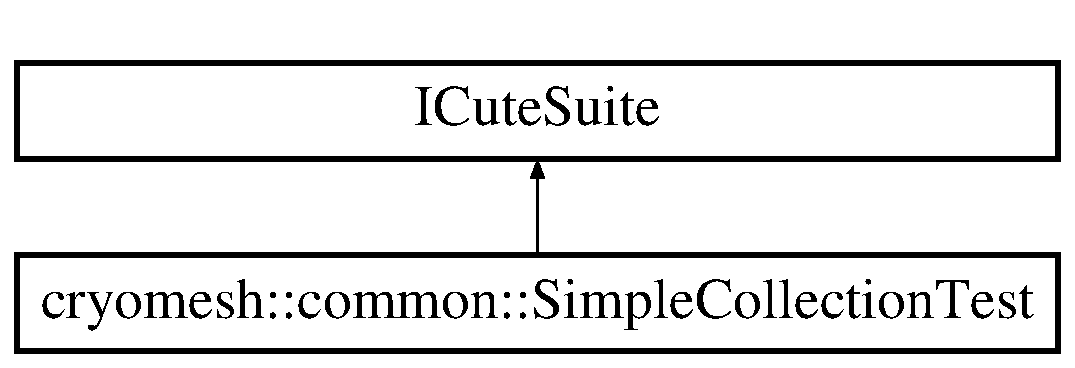
\includegraphics[height=2.000000cm]{classcryomesh_1_1common_1_1_simple_collection_test}
\end{center}
\end{figure}
\subsection*{Public Member Functions}
\begin{DoxyCompactItemize}
\item 
virtual \hyperlink{classcryomesh_1_1common_1_1_simple_collection_test_abb9151f771142f0f40f92e2c57bb99f0}{$\sim$SimpleCollectionTest} ()
\end{DoxyCompactItemize}
\subsection*{Static Public Member Functions}
\begin{DoxyCompactItemize}
\item 
static void \hyperlink{classcryomesh_1_1common_1_1_simple_collection_test_aa79c9251cc90f5fb52774cccddfa3b96}{runSuite} ()
\item 
static void \hyperlink{classcryomesh_1_1common_1_1_simple_collection_test_a5497e957f4c59796388400eb01883035}{testAddRemove} ()
\item 
static void \hyperlink{classcryomesh_1_1common_1_1_simple_collection_test_a9cfeecaf8cbfc318d38a48c81ba61913}{testSum} ()
\item 
static void \hyperlink{classcryomesh_1_1common_1_1_simple_collection_test_a26c158f89bdc84f4cf1f1ed6874321d1}{testMaxMin} ()
\item 
static void \hyperlink{classcryomesh_1_1common_1_1_simple_collection_test_a47cfd0be3864fd8452d53bd0a2bc15ae}{testGetValueAt} ()
\item 
static void \hyperlink{classcryomesh_1_1common_1_1_simple_collection_test_aa591e7768584f7c8a3d99a62839f4883}{testInverseReverse} ()
\item 
static void \hyperlink{classcryomesh_1_1common_1_1_simple_collection_test_ae7f95badd9de7271bc0e746fbaa42706}{testOperators} ()
\item 
static void \hyperlink{classcryomesh_1_1common_1_1_simple_collection_test_aa77eb7323a6f46dc1f9fc47c03278f2b}{testPad} ()
\end{DoxyCompactItemize}
\subsection*{Protected Member Functions}
\begin{DoxyCompactItemize}
\item 
\hyperlink{classcryomesh_1_1common_1_1_simple_collection_test_ab40867505de8fe8abddc70027f491a04}{SimpleCollectionTest} ()
\end{DoxyCompactItemize}


\subsection{Constructor \& Destructor Documentation}
\hypertarget{classcryomesh_1_1common_1_1_simple_collection_test_abb9151f771142f0f40f92e2c57bb99f0}{
\index{cryomesh::common::SimpleCollectionTest@{cryomesh::common::SimpleCollectionTest}!$\sim$SimpleCollectionTest@{$\sim$SimpleCollectionTest}}
\index{$\sim$SimpleCollectionTest@{$\sim$SimpleCollectionTest}!cryomesh::common::SimpleCollectionTest@{cryomesh::common::SimpleCollectionTest}}
\subsubsection[{$\sim$SimpleCollectionTest}]{\setlength{\rightskip}{0pt plus 5cm}cryomesh::common::SimpleCollectionTest::$\sim$SimpleCollectionTest (
\begin{DoxyParamCaption}
{}
\end{DoxyParamCaption}
)\hspace{0.3cm}{\ttfamily  \mbox{[}virtual\mbox{]}}}}
\label{classcryomesh_1_1common_1_1_simple_collection_test_abb9151f771142f0f40f92e2c57bb99f0}
Destructor \hypertarget{classcryomesh_1_1common_1_1_simple_collection_test_ab40867505de8fe8abddc70027f491a04}{
\index{cryomesh::common::SimpleCollectionTest@{cryomesh::common::SimpleCollectionTest}!SimpleCollectionTest@{SimpleCollectionTest}}
\index{SimpleCollectionTest@{SimpleCollectionTest}!cryomesh::common::SimpleCollectionTest@{cryomesh::common::SimpleCollectionTest}}
\subsubsection[{SimpleCollectionTest}]{\setlength{\rightskip}{0pt plus 5cm}cryomesh::common::SimpleCollectionTest::SimpleCollectionTest (
\begin{DoxyParamCaption}
{}
\end{DoxyParamCaption}
)\hspace{0.3cm}{\ttfamily  \mbox{[}protected\mbox{]}}}}
\label{classcryomesh_1_1common_1_1_simple_collection_test_ab40867505de8fe8abddc70027f491a04}
Protected contructor to prevent initialisation 

\subsection{Member Function Documentation}
\hypertarget{classcryomesh_1_1common_1_1_simple_collection_test_aa79c9251cc90f5fb52774cccddfa3b96}{
\index{cryomesh::common::SimpleCollectionTest@{cryomesh::common::SimpleCollectionTest}!runSuite@{runSuite}}
\index{runSuite@{runSuite}!cryomesh::common::SimpleCollectionTest@{cryomesh::common::SimpleCollectionTest}}
\subsubsection[{runSuite}]{\setlength{\rightskip}{0pt plus 5cm}void cryomesh::common::SimpleCollectionTest::runSuite (
\begin{DoxyParamCaption}
{}
\end{DoxyParamCaption}
)\hspace{0.3cm}{\ttfamily  \mbox{[}static\mbox{]}}}}
\label{classcryomesh_1_1common_1_1_simple_collection_test_aa79c9251cc90f5fb52774cccddfa3b96}
Run all tests \hypertarget{classcryomesh_1_1common_1_1_simple_collection_test_a5497e957f4c59796388400eb01883035}{
\index{cryomesh::common::SimpleCollectionTest@{cryomesh::common::SimpleCollectionTest}!testAddRemove@{testAddRemove}}
\index{testAddRemove@{testAddRemove}!cryomesh::common::SimpleCollectionTest@{cryomesh::common::SimpleCollectionTest}}
\subsubsection[{testAddRemove}]{\setlength{\rightskip}{0pt plus 5cm}void cryomesh::common::SimpleCollectionTest::testAddRemove (
\begin{DoxyParamCaption}
{}
\end{DoxyParamCaption}
)\hspace{0.3cm}{\ttfamily  \mbox{[}static\mbox{]}}}}
\label{classcryomesh_1_1common_1_1_simple_collection_test_a5497e957f4c59796388400eb01883035}
Test adding and removing elements \hypertarget{classcryomesh_1_1common_1_1_simple_collection_test_a47cfd0be3864fd8452d53bd0a2bc15ae}{
\index{cryomesh::common::SimpleCollectionTest@{cryomesh::common::SimpleCollectionTest}!testGetValueAt@{testGetValueAt}}
\index{testGetValueAt@{testGetValueAt}!cryomesh::common::SimpleCollectionTest@{cryomesh::common::SimpleCollectionTest}}
\subsubsection[{testGetValueAt}]{\setlength{\rightskip}{0pt plus 5cm}void cryomesh::common::SimpleCollectionTest::testGetValueAt (
\begin{DoxyParamCaption}
{}
\end{DoxyParamCaption}
)\hspace{0.3cm}{\ttfamily  \mbox{[}static\mbox{]}}}}
\label{classcryomesh_1_1common_1_1_simple_collection_test_a47cfd0be3864fd8452d53bd0a2bc15ae}
Test getting value by index \hypertarget{classcryomesh_1_1common_1_1_simple_collection_test_aa591e7768584f7c8a3d99a62839f4883}{
\index{cryomesh::common::SimpleCollectionTest@{cryomesh::common::SimpleCollectionTest}!testInverseReverse@{testInverseReverse}}
\index{testInverseReverse@{testInverseReverse}!cryomesh::common::SimpleCollectionTest@{cryomesh::common::SimpleCollectionTest}}
\subsubsection[{testInverseReverse}]{\setlength{\rightskip}{0pt plus 5cm}void cryomesh::common::SimpleCollectionTest::testInverseReverse (
\begin{DoxyParamCaption}
{}
\end{DoxyParamCaption}
)\hspace{0.3cm}{\ttfamily  \mbox{[}static\mbox{]}}}}
\label{classcryomesh_1_1common_1_1_simple_collection_test_aa591e7768584f7c8a3d99a62839f4883}
test inverting and reversing \hypertarget{classcryomesh_1_1common_1_1_simple_collection_test_a26c158f89bdc84f4cf1f1ed6874321d1}{
\index{cryomesh::common::SimpleCollectionTest@{cryomesh::common::SimpleCollectionTest}!testMaxMin@{testMaxMin}}
\index{testMaxMin@{testMaxMin}!cryomesh::common::SimpleCollectionTest@{cryomesh::common::SimpleCollectionTest}}
\subsubsection[{testMaxMin}]{\setlength{\rightskip}{0pt plus 5cm}void cryomesh::common::SimpleCollectionTest::testMaxMin (
\begin{DoxyParamCaption}
{}
\end{DoxyParamCaption}
)\hspace{0.3cm}{\ttfamily  \mbox{[}static\mbox{]}}}}
\label{classcryomesh_1_1common_1_1_simple_collection_test_a26c158f89bdc84f4cf1f1ed6874321d1}
Test getting maximum and minimum values \hypertarget{classcryomesh_1_1common_1_1_simple_collection_test_ae7f95badd9de7271bc0e746fbaa42706}{
\index{cryomesh::common::SimpleCollectionTest@{cryomesh::common::SimpleCollectionTest}!testOperators@{testOperators}}
\index{testOperators@{testOperators}!cryomesh::common::SimpleCollectionTest@{cryomesh::common::SimpleCollectionTest}}
\subsubsection[{testOperators}]{\setlength{\rightskip}{0pt plus 5cm}void cryomesh::common::SimpleCollectionTest::testOperators (
\begin{DoxyParamCaption}
{}
\end{DoxyParamCaption}
)\hspace{0.3cm}{\ttfamily  \mbox{[}static\mbox{]}}}}
\label{classcryomesh_1_1common_1_1_simple_collection_test_ae7f95badd9de7271bc0e746fbaa42706}
Test all operators \hypertarget{classcryomesh_1_1common_1_1_simple_collection_test_aa77eb7323a6f46dc1f9fc47c03278f2b}{
\index{cryomesh::common::SimpleCollectionTest@{cryomesh::common::SimpleCollectionTest}!testPad@{testPad}}
\index{testPad@{testPad}!cryomesh::common::SimpleCollectionTest@{cryomesh::common::SimpleCollectionTest}}
\subsubsection[{testPad}]{\setlength{\rightskip}{0pt plus 5cm}void cryomesh::common::SimpleCollectionTest::testPad (
\begin{DoxyParamCaption}
{}
\end{DoxyParamCaption}
)\hspace{0.3cm}{\ttfamily  \mbox{[}static\mbox{]}}}}
\label{classcryomesh_1_1common_1_1_simple_collection_test_aa77eb7323a6f46dc1f9fc47c03278f2b}
Test padding collections \hypertarget{classcryomesh_1_1common_1_1_simple_collection_test_a9cfeecaf8cbfc318d38a48c81ba61913}{
\index{cryomesh::common::SimpleCollectionTest@{cryomesh::common::SimpleCollectionTest}!testSum@{testSum}}
\index{testSum@{testSum}!cryomesh::common::SimpleCollectionTest@{cryomesh::common::SimpleCollectionTest}}
\subsubsection[{testSum}]{\setlength{\rightskip}{0pt plus 5cm}void cryomesh::common::SimpleCollectionTest::testSum (
\begin{DoxyParamCaption}
{}
\end{DoxyParamCaption}
)\hspace{0.3cm}{\ttfamily  \mbox{[}static\mbox{]}}}}
\label{classcryomesh_1_1common_1_1_simple_collection_test_a9cfeecaf8cbfc318d38a48c81ba61913}
Test getting sum of all elements 

The documentation for this class was generated from the following files:\begin{DoxyCompactItemize}
\item 
src/common/\hyperlink{_simple_collection_test_8h}{SimpleCollectionTest.h}\item 
src/common/\hyperlink{_simple_collection_test_8cpp}{SimpleCollectionTest.cpp}\end{DoxyCompactItemize}

\hypertarget{classcryomesh_1_1_test_templates}{
\section{cryomesh::TestTemplates Class Reference}
\label{classcryomesh_1_1_test_templates}\index{cryomesh::TestTemplates@{cryomesh::TestTemplates}}
}


{\ttfamily \#include $<$TestTemplates.h$>$}

\subsection*{Public Member Functions}
\begin{DoxyCompactItemize}
\item 
\hyperlink{classcryomesh_1_1_test_templates_ae20dd77451376780e6e0f37dfc9f6088}{TestTemplates} ()
\item 
virtual \hyperlink{classcryomesh_1_1_test_templates_a959cf0d7cd43e19dc553cab3e3db2beb}{$\sim$TestTemplates} ()
\end{DoxyCompactItemize}


\subsection{Constructor \& Destructor Documentation}
\hypertarget{classcryomesh_1_1_test_templates_ae20dd77451376780e6e0f37dfc9f6088}{
\index{cryomesh::TestTemplates@{cryomesh::TestTemplates}!TestTemplates@{TestTemplates}}
\index{TestTemplates@{TestTemplates}!cryomesh::TestTemplates@{cryomesh::TestTemplates}}
\subsubsection[{TestTemplates}]{\setlength{\rightskip}{0pt plus 5cm}cryomesh::TestTemplates::TestTemplates (
\begin{DoxyParamCaption}
{}
\end{DoxyParamCaption}
)}}
\label{classcryomesh_1_1_test_templates_ae20dd77451376780e6e0f37dfc9f6088}
\hypertarget{classcryomesh_1_1_test_templates_a959cf0d7cd43e19dc553cab3e3db2beb}{
\index{cryomesh::TestTemplates@{cryomesh::TestTemplates}!$\sim$TestTemplates@{$\sim$TestTemplates}}
\index{$\sim$TestTemplates@{$\sim$TestTemplates}!cryomesh::TestTemplates@{cryomesh::TestTemplates}}
\subsubsection[{$\sim$TestTemplates}]{\setlength{\rightskip}{0pt plus 5cm}virtual cryomesh::TestTemplates::$\sim$TestTemplates (
\begin{DoxyParamCaption}
{}
\end{DoxyParamCaption}
)\hspace{0.3cm}{\ttfamily  \mbox{[}virtual\mbox{]}}}}
\label{classcryomesh_1_1_test_templates_a959cf0d7cd43e19dc553cab3e3db2beb}


The documentation for this class was generated from the following file:\begin{DoxyCompactItemize}
\item 
src/\hyperlink{_test_templates_8h}{TestTemplates.h}\end{DoxyCompactItemize}

\hypertarget{classcryomesh_1_1common_1_1_time_keeper_test}{
\section{cryomesh::common::TimeKeeperTest Class Reference}
\label{classcryomesh_1_1common_1_1_time_keeper_test}\index{cryomesh::common::TimeKeeperTest@{cryomesh::common::TimeKeeperTest}}
}


{\ttfamily \#include $<$TimeKeeperTest.h$>$}

\subsection*{Static Public Member Functions}
\begin{DoxyCompactItemize}
\item 
static void \hyperlink{classcryomesh_1_1common_1_1_time_keeper_test_a33e9aabb114393a14fa3fdaaae5954f2}{runSuite} ()
\item 
static void \hyperlink{classcryomesh_1_1common_1_1_time_keeper_test_ade7f64b633ec6b7f5bb33244c6a99354}{testserialize} ()
\item 
static void \hyperlink{classcryomesh_1_1common_1_1_time_keeper_test_aa27cea26c5d307be18d72537a32b369d}{testTimeKeeper} ()
\item 
static void \hyperlink{classcryomesh_1_1common_1_1_time_keeper_test_a26191e841ffcbf2a28907bd3ca9cbb28}{testupdate} ()
\item 
static void \hyperlink{classcryomesh_1_1common_1_1_time_keeper_test_a32e20cfa590549737e4eef71cd85a3fe}{testgetCycle} ()
\item 
static void \hyperlink{classcryomesh_1_1common_1_1_time_keeper_test_adde2577c9f9af996f8d20e5c8a75a528}{testgetTiming} ()
\end{DoxyCompactItemize}


\subsection{Member Function Documentation}
\hypertarget{classcryomesh_1_1common_1_1_time_keeper_test_a33e9aabb114393a14fa3fdaaae5954f2}{
\index{cryomesh::common::TimeKeeperTest@{cryomesh::common::TimeKeeperTest}!runSuite@{runSuite}}
\index{runSuite@{runSuite}!cryomesh::common::TimeKeeperTest@{cryomesh::common::TimeKeeperTest}}
\subsubsection[{runSuite}]{\setlength{\rightskip}{0pt plus 5cm}void cryomesh::common::TimeKeeperTest::runSuite (
\begin{DoxyParamCaption}
{}
\end{DoxyParamCaption}
)\hspace{0.3cm}{\ttfamily  \mbox{[}static\mbox{]}}}}
\label{classcryomesh_1_1common_1_1_time_keeper_test_a33e9aabb114393a14fa3fdaaae5954f2}
\hypertarget{classcryomesh_1_1common_1_1_time_keeper_test_a32e20cfa590549737e4eef71cd85a3fe}{
\index{cryomesh::common::TimeKeeperTest@{cryomesh::common::TimeKeeperTest}!testgetCycle@{testgetCycle}}
\index{testgetCycle@{testgetCycle}!cryomesh::common::TimeKeeperTest@{cryomesh::common::TimeKeeperTest}}
\subsubsection[{testgetCycle}]{\setlength{\rightskip}{0pt plus 5cm}void cryomesh::common::TimeKeeperTest::testgetCycle (
\begin{DoxyParamCaption}
{}
\end{DoxyParamCaption}
)\hspace{0.3cm}{\ttfamily  \mbox{[}static\mbox{]}}}}
\label{classcryomesh_1_1common_1_1_time_keeper_test_a32e20cfa590549737e4eef71cd85a3fe}
\hypertarget{classcryomesh_1_1common_1_1_time_keeper_test_adde2577c9f9af996f8d20e5c8a75a528}{
\index{cryomesh::common::TimeKeeperTest@{cryomesh::common::TimeKeeperTest}!testgetTiming@{testgetTiming}}
\index{testgetTiming@{testgetTiming}!cryomesh::common::TimeKeeperTest@{cryomesh::common::TimeKeeperTest}}
\subsubsection[{testgetTiming}]{\setlength{\rightskip}{0pt plus 5cm}void cryomesh::common::TimeKeeperTest::testgetTiming (
\begin{DoxyParamCaption}
{}
\end{DoxyParamCaption}
)\hspace{0.3cm}{\ttfamily  \mbox{[}static\mbox{]}}}}
\label{classcryomesh_1_1common_1_1_time_keeper_test_adde2577c9f9af996f8d20e5c8a75a528}
\hypertarget{classcryomesh_1_1common_1_1_time_keeper_test_ade7f64b633ec6b7f5bb33244c6a99354}{
\index{cryomesh::common::TimeKeeperTest@{cryomesh::common::TimeKeeperTest}!testserialize@{testserialize}}
\index{testserialize@{testserialize}!cryomesh::common::TimeKeeperTest@{cryomesh::common::TimeKeeperTest}}
\subsubsection[{testserialize}]{\setlength{\rightskip}{0pt plus 5cm}void cryomesh::common::TimeKeeperTest::testserialize (
\begin{DoxyParamCaption}
{}
\end{DoxyParamCaption}
)\hspace{0.3cm}{\ttfamily  \mbox{[}static\mbox{]}}}}
\label{classcryomesh_1_1common_1_1_time_keeper_test_ade7f64b633ec6b7f5bb33244c6a99354}
\hypertarget{classcryomesh_1_1common_1_1_time_keeper_test_aa27cea26c5d307be18d72537a32b369d}{
\index{cryomesh::common::TimeKeeperTest@{cryomesh::common::TimeKeeperTest}!testTimeKeeper@{testTimeKeeper}}
\index{testTimeKeeper@{testTimeKeeper}!cryomesh::common::TimeKeeperTest@{cryomesh::common::TimeKeeperTest}}
\subsubsection[{testTimeKeeper}]{\setlength{\rightskip}{0pt plus 5cm}void cryomesh::common::TimeKeeperTest::testTimeKeeper (
\begin{DoxyParamCaption}
{}
\end{DoxyParamCaption}
)\hspace{0.3cm}{\ttfamily  \mbox{[}static\mbox{]}}}}
\label{classcryomesh_1_1common_1_1_time_keeper_test_aa27cea26c5d307be18d72537a32b369d}
\hypertarget{classcryomesh_1_1common_1_1_time_keeper_test_a26191e841ffcbf2a28907bd3ca9cbb28}{
\index{cryomesh::common::TimeKeeperTest@{cryomesh::common::TimeKeeperTest}!testupdate@{testupdate}}
\index{testupdate@{testupdate}!cryomesh::common::TimeKeeperTest@{cryomesh::common::TimeKeeperTest}}
\subsubsection[{testupdate}]{\setlength{\rightskip}{0pt plus 5cm}void cryomesh::common::TimeKeeperTest::testupdate (
\begin{DoxyParamCaption}
{}
\end{DoxyParamCaption}
)\hspace{0.3cm}{\ttfamily  \mbox{[}static\mbox{]}}}}
\label{classcryomesh_1_1common_1_1_time_keeper_test_a26191e841ffcbf2a28907bd3ca9cbb28}


The documentation for this class was generated from the following files:\begin{DoxyCompactItemize}
\item 
src/common/\hyperlink{_time_keeper_test_8h}{TimeKeeperTest.h}\item 
src/common/\hyperlink{_time_keeper_test_8cpp}{TimeKeeperTest.cpp}\end{DoxyCompactItemize}

\hypertarget{classcryomesh_1_1components_1_1_use_case_impulse_propagation}{
\section{cryomesh::components::UseCaseImpulsePropagation Class Reference}
\label{classcryomesh_1_1components_1_1_use_case_impulse_propagation}\index{cryomesh::components::UseCaseImpulsePropagation@{cryomesh::components::UseCaseImpulsePropagation}}
}


{\ttfamily \#include $<$UseCaseImpulsePropagation.h$>$}

Inheritance diagram for cryomesh::components::UseCaseImpulsePropagation:\begin{figure}[H]
\begin{center}
\leavevmode
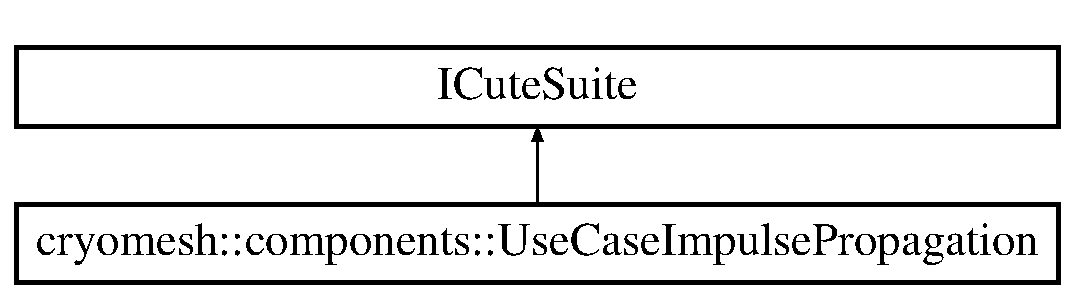
\includegraphics[height=2.000000cm]{classcryomesh_1_1components_1_1_use_case_impulse_propagation}
\end{center}
\end{figure}
\subsection*{Public Member Functions}
\begin{DoxyCompactItemize}
\item 
virtual \hyperlink{classcryomesh_1_1components_1_1_use_case_impulse_propagation_a8cdcc2f6e0fc9af7711972a75e2fe006}{$\sim$UseCaseImpulsePropagation} ()
\end{DoxyCompactItemize}
\subsection*{Static Public Member Functions}
\begin{DoxyCompactItemize}
\item 
static void \hyperlink{classcryomesh_1_1components_1_1_use_case_impulse_propagation_ad978f981b7f2164efb58f96b640c3faa}{runSuite} ()
\item 
static void \hyperlink{classcryomesh_1_1components_1_1_use_case_impulse_propagation_aa6101422117b1b83ce04fe087a669ff2}{testPropagation} ()
\end{DoxyCompactItemize}
\subsection*{Protected Member Functions}
\begin{DoxyCompactItemize}
\item 
\hyperlink{classcryomesh_1_1components_1_1_use_case_impulse_propagation_abe368a0fe2b1f9f51c5d1ad15815279e}{UseCaseImpulsePropagation} ()
\end{DoxyCompactItemize}


\subsection{Detailed Description}
Use case test of propagation from a Node, through a Connections and ending in a Node again 

\subsection{Constructor \& Destructor Documentation}
\hypertarget{classcryomesh_1_1components_1_1_use_case_impulse_propagation_a8cdcc2f6e0fc9af7711972a75e2fe006}{
\index{cryomesh::components::UseCaseImpulsePropagation@{cryomesh::components::UseCaseImpulsePropagation}!$\sim$UseCaseImpulsePropagation@{$\sim$UseCaseImpulsePropagation}}
\index{$\sim$UseCaseImpulsePropagation@{$\sim$UseCaseImpulsePropagation}!cryomesh::components::UseCaseImpulsePropagation@{cryomesh::components::UseCaseImpulsePropagation}}
\subsubsection[{$\sim$UseCaseImpulsePropagation}]{\setlength{\rightskip}{0pt plus 5cm}virtual cryomesh::components::UseCaseImpulsePropagation::$\sim$UseCaseImpulsePropagation (
\begin{DoxyParamCaption}
{}
\end{DoxyParamCaption}
)\hspace{0.3cm}{\ttfamily  \mbox{[}inline, virtual\mbox{]}}}}
\label{classcryomesh_1_1components_1_1_use_case_impulse_propagation_a8cdcc2f6e0fc9af7711972a75e2fe006}
\hypertarget{classcryomesh_1_1components_1_1_use_case_impulse_propagation_abe368a0fe2b1f9f51c5d1ad15815279e}{
\index{cryomesh::components::UseCaseImpulsePropagation@{cryomesh::components::UseCaseImpulsePropagation}!UseCaseImpulsePropagation@{UseCaseImpulsePropagation}}
\index{UseCaseImpulsePropagation@{UseCaseImpulsePropagation}!cryomesh::components::UseCaseImpulsePropagation@{cryomesh::components::UseCaseImpulsePropagation}}
\subsubsection[{UseCaseImpulsePropagation}]{\setlength{\rightskip}{0pt plus 5cm}cryomesh::components::UseCaseImpulsePropagation::UseCaseImpulsePropagation (
\begin{DoxyParamCaption}
{}
\end{DoxyParamCaption}
)\hspace{0.3cm}{\ttfamily  \mbox{[}inline, protected\mbox{]}}}}
\label{classcryomesh_1_1components_1_1_use_case_impulse_propagation_abe368a0fe2b1f9f51c5d1ad15815279e}


\subsection{Member Function Documentation}
\hypertarget{classcryomesh_1_1components_1_1_use_case_impulse_propagation_ad978f981b7f2164efb58f96b640c3faa}{
\index{cryomesh::components::UseCaseImpulsePropagation@{cryomesh::components::UseCaseImpulsePropagation}!runSuite@{runSuite}}
\index{runSuite@{runSuite}!cryomesh::components::UseCaseImpulsePropagation@{cryomesh::components::UseCaseImpulsePropagation}}
\subsubsection[{runSuite}]{\setlength{\rightskip}{0pt plus 5cm}void cryomesh::components::UseCaseImpulsePropagation::runSuite (
\begin{DoxyParamCaption}
{}
\end{DoxyParamCaption}
)\hspace{0.3cm}{\ttfamily  \mbox{[}static\mbox{]}}}}
\label{classcryomesh_1_1components_1_1_use_case_impulse_propagation_ad978f981b7f2164efb58f96b640c3faa}
Run all tests \hypertarget{classcryomesh_1_1components_1_1_use_case_impulse_propagation_aa6101422117b1b83ce04fe087a669ff2}{
\index{cryomesh::components::UseCaseImpulsePropagation@{cryomesh::components::UseCaseImpulsePropagation}!testPropagation@{testPropagation}}
\index{testPropagation@{testPropagation}!cryomesh::components::UseCaseImpulsePropagation@{cryomesh::components::UseCaseImpulsePropagation}}
\subsubsection[{testPropagation}]{\setlength{\rightskip}{0pt plus 5cm}void cryomesh::components::UseCaseImpulsePropagation::testPropagation (
\begin{DoxyParamCaption}
{}
\end{DoxyParamCaption}
)\hspace{0.3cm}{\ttfamily  \mbox{[}static\mbox{]}}}}
\label{classcryomesh_1_1components_1_1_use_case_impulse_propagation_aa6101422117b1b83ce04fe087a669ff2}
Test propagation through nodes and connections 

The documentation for this class was generated from the following files:\begin{DoxyCompactItemize}
\item 
src/components/\hyperlink{_use_case_impulse_propagation_8h}{UseCaseImpulsePropagation.h}\item 
src/components/\hyperlink{_use_case_impulse_propagation_8cpp}{UseCaseImpulsePropagation.cpp}\end{DoxyCompactItemize}

\chapter{File Documentation}
\hypertarget{_connector_test_8cpp}{
\section{src/common/ConnectorTest.cpp File Reference}
\label{_connector_test_8cpp}\index{src/common/ConnectorTest.cpp@{src/common/ConnectorTest.cpp}}
}
{\ttfamily \#include \char`\"{}ConnectorTest.h\char`\"{}}\par
\subsection*{Namespaces}
\begin{DoxyCompactItemize}
\item 
namespace \hyperlink{namespacecryomesh}{cryomesh}
\item 
namespace \hyperlink{namespacecryomesh_1_1common}{cryomesh::common}
\end{DoxyCompactItemize}

\hypertarget{_connector_test_8h}{
\section{src/common/ConnectorTest.h File Reference}
\label{_connector_test_8h}\index{src/common/ConnectorTest.h@{src/common/ConnectorTest.h}}
}
{\ttfamily \#include \char`\"{}ICuteSuite.h\char`\"{}}\par
{\ttfamily \#include \char`\"{}common/Connector.h\char`\"{}}\par
{\ttfamily \#include \char`\"{}components/Connection.h\char`\"{}}\par
{\ttfamily \#include \char`\"{}components/Node.h\char`\"{}}\par
\subsection*{Classes}
\begin{DoxyCompactItemize}
\item 
class \hyperlink{classcryomesh_1_1common_1_1_connector_test}{cryomesh::common::ConnectorTest}
\end{DoxyCompactItemize}
\subsection*{Namespaces}
\begin{DoxyCompactItemize}
\item 
namespace \hyperlink{namespacecryomesh}{cryomesh}
\item 
namespace \hyperlink{namespacecryomesh_1_1common}{cryomesh::common}
\end{DoxyCompactItemize}

\hypertarget{_containers_test_8cpp}{
\section{src/common/ContainersTest.cpp File Reference}
\label{_containers_test_8cpp}\index{src/common/ContainersTest.cpp@{src/common/ContainersTest.cpp}}
}
{\ttfamily \#include \char`\"{}ContainersTest.h\char`\"{}}\par
{\ttfamily \#include \char`\"{}common/Containers.h\char`\"{}}\par
\subsection*{Namespaces}
\begin{DoxyCompactItemize}
\item 
namespace \hyperlink{namespacecryomesh}{cryomesh}
\item 
namespace \hyperlink{namespacecryomesh_1_1common}{cryomesh::common}
\end{DoxyCompactItemize}

\hypertarget{_containers_test_8h}{
\section{src/common/ContainersTest.h File Reference}
\label{_containers_test_8h}\index{src/common/ContainersTest.h@{src/common/ContainersTest.h}}
}
{\ttfamily \#include \char`\"{}ICuteSuite.h\char`\"{}}\par
\subsection*{Classes}
\begin{DoxyCompactItemize}
\item 
class \hyperlink{classcryomesh_1_1common_1_1_containers_test}{cryomesh::common::ContainersTest}
\end{DoxyCompactItemize}
\subsection*{Namespaces}
\begin{DoxyCompactItemize}
\item 
namespace \hyperlink{namespacecryomesh}{cryomesh}
\item 
namespace \hyperlink{namespacecryomesh_1_1common}{cryomesh::common}
\end{DoxyCompactItemize}

\hypertarget{_maths_test_8cpp}{
\section{src/common/MathsTest.cpp File Reference}
\label{_maths_test_8cpp}\index{src/common/MathsTest.cpp@{src/common/MathsTest.cpp}}
}
{\ttfamily \#include \char`\"{}MathsTest.h\char`\"{}}\par
{\ttfamily \#include \char`\"{}common/Maths.h\char`\"{}}\par
{\ttfamily \#include $<$ctime$>$}\par
\subsection*{Namespaces}
\begin{DoxyCompactItemize}
\item 
namespace \hyperlink{namespacecryomesh}{cryomesh}
\item 
namespace \hyperlink{namespacecryomesh_1_1common}{cryomesh::common}
\end{DoxyCompactItemize}

\hypertarget{_maths_test_8h}{
\section{src/common/MathsTest.h File Reference}
\label{_maths_test_8h}\index{src/common/MathsTest.h@{src/common/MathsTest.h}}
}
{\ttfamily \#include \char`\"{}ICuteSuite.h\char`\"{}}\par
\subsection*{Classes}
\begin{DoxyCompactItemize}
\item 
class \hyperlink{classcryomesh_1_1common_1_1_maths_test}{cryomesh::common::MathsTest}
\end{DoxyCompactItemize}
\subsection*{Namespaces}
\begin{DoxyCompactItemize}
\item 
namespace \hyperlink{namespacecryomesh}{cryomesh}
\item 
namespace \hyperlink{namespacecryomesh_1_1common}{cryomesh::common}
\end{DoxyCompactItemize}

\hypertarget{_misc_test_8cpp}{
\section{src/common/MiscTest.cpp File Reference}
\label{_misc_test_8cpp}\index{src/common/MiscTest.cpp@{src/common/MiscTest.cpp}}
}
{\ttfamily \#include \char`\"{}MiscTest.h\char`\"{}}\par
\subsection*{Namespaces}
\begin{DoxyCompactItemize}
\item 
namespace \hyperlink{namespacecryomesh}{cryomesh}
\item 
namespace \hyperlink{namespacecryomesh_1_1common}{cryomesh::common}
\end{DoxyCompactItemize}

\hypertarget{_misc_test_8h}{
\section{src/common/MiscTest.h File Reference}
\label{_misc_test_8h}\index{src/common/MiscTest.h@{src/common/MiscTest.h}}
}
{\ttfamily \#include $<$boost/shared\_\-ptr.hpp$>$}\par
{\ttfamily \#include \char`\"{}common/Misc.h\char`\"{}}\par
{\ttfamily \#include \char`\"{}ICuteSuite.h\char`\"{}}\par
\subsection*{Classes}
\begin{DoxyCompactItemize}
\item 
class \hyperlink{classcryomesh_1_1common_1_1_misc_test}{cryomesh::common::MiscTest}
\end{DoxyCompactItemize}
\subsection*{Namespaces}
\begin{DoxyCompactItemize}
\item 
namespace \hyperlink{namespacecryomesh}{cryomesh}
\item 
namespace \hyperlink{namespacecryomesh_1_1common}{cryomesh::common}
\end{DoxyCompactItemize}

\hypertarget{_simple_collection_test_8cpp}{
\section{src/common/SimpleCollectionTest.cpp File Reference}
\label{_simple_collection_test_8cpp}\index{src/common/SimpleCollectionTest.cpp@{src/common/SimpleCollectionTest.cpp}}
}
{\ttfamily \#include \char`\"{}SimpleCollectionTest.h\char`\"{}}\par
{\ttfamily \#include \char`\"{}common/SimpleCollection.h\char`\"{}}\par
\subsection*{Namespaces}
\begin{DoxyCompactItemize}
\item 
namespace \hyperlink{namespacecryomesh}{cryomesh}
\item 
namespace \hyperlink{namespacecryomesh_1_1common}{cryomesh::common}
\end{DoxyCompactItemize}

\hypertarget{_simple_collection_test_8h}{
\section{src/common/SimpleCollectionTest.h File Reference}
\label{_simple_collection_test_8h}\index{src/common/SimpleCollectionTest.h@{src/common/SimpleCollectionTest.h}}
}
{\ttfamily \#include \char`\"{}ICuteSuite.h\char`\"{}}\par
\subsection*{Classes}
\begin{DoxyCompactItemize}
\item 
class \hyperlink{classcryomesh_1_1common_1_1_simple_collection_test}{cryomesh::common::SimpleCollectionTest}
\end{DoxyCompactItemize}
\subsection*{Namespaces}
\begin{DoxyCompactItemize}
\item 
namespace \hyperlink{namespacecryomesh}{cryomesh}
\item 
namespace \hyperlink{namespacecryomesh_1_1common}{cryomesh::common}
\end{DoxyCompactItemize}

\hypertarget{_time_keeper_test_8cpp}{
\section{src/common/TimeKeeperTest.cpp File Reference}
\label{_time_keeper_test_8cpp}\index{src/common/TimeKeeperTest.cpp@{src/common/TimeKeeperTest.cpp}}
}
{\ttfamily \#include \char`\"{}TimeKeeperTest.h\char`\"{}}\par
{\ttfamily \#include \char`\"{}cute.h\char`\"{}}\par
{\ttfamily \#include \char`\"{}ide\_\-listener.h\char`\"{}}\par
{\ttfamily \#include \char`\"{}cute\_\-runner.h\char`\"{}}\par
{\ttfamily \#include $<$fstream$>$}\par
\subsection*{Namespaces}
\begin{DoxyCompactItemize}
\item 
namespace \hyperlink{namespacecryomesh}{cryomesh}
\item 
namespace \hyperlink{namespacecryomesh_1_1common}{cryomesh::common}
\end{DoxyCompactItemize}

\hypertarget{_time_keeper_test_8h}{
\section{src/common/TimeKeeperTest.h File Reference}
\label{_time_keeper_test_8h}\index{src/common/TimeKeeperTest.h@{src/common/TimeKeeperTest.h}}
}
{\ttfamily \#include \char`\"{}common/TimeKeeper.h\char`\"{}}\par
{\ttfamily \#include \char`\"{}CoreTestsDefaults.h\char`\"{}}\par
{\ttfamily \#include $<$boost/archive/text\_\-iarchive.hpp$>$}\par
{\ttfamily \#include $<$boost/archive/text\_\-oarchive.hpp$>$}\par
\subsection*{Classes}
\begin{DoxyCompactItemize}
\item 
class \hyperlink{classcryomesh_1_1common_1_1_time_keeper_test}{cryomesh::common::TimeKeeperTest}
\end{DoxyCompactItemize}
\subsection*{Namespaces}
\begin{DoxyCompactItemize}
\item 
namespace \hyperlink{namespacecryomesh}{cryomesh}
\item 
namespace \hyperlink{namespacecryomesh_1_1common}{cryomesh::common}
\end{DoxyCompactItemize}

\hypertarget{_impulse_collection_test_8cpp}{
\section{src/components/ImpulseCollectionTest.cpp File Reference}
\label{_impulse_collection_test_8cpp}\index{src/components/ImpulseCollectionTest.cpp@{src/components/ImpulseCollectionTest.cpp}}
}
{\ttfamily \#include \char`\"{}ImpulseCollectionTest.h\char`\"{}}\par
{\ttfamily \#include \char`\"{}components/Mesh.h\char`\"{}}\par
{\ttfamily \#include \char`\"{}components/ImpulseCollection.h\char`\"{}}\par
{\ttfamily \#include \char`\"{}common/TimeKeeper.h\char`\"{}}\par
\subsection*{Namespaces}
\begin{DoxyCompactItemize}
\item 
namespace \hyperlink{namespacecryomesh}{cryomesh}
\item 
namespace \hyperlink{namespacecryomesh_1_1components}{cryomesh::components}
\end{DoxyCompactItemize}

\hypertarget{_impulse_collection_test_8h}{
\section{src/components/ImpulseCollectionTest.h File Reference}
\label{_impulse_collection_test_8h}\index{src/components/ImpulseCollectionTest.h@{src/components/ImpulseCollectionTest.h}}
}
{\ttfamily \#include \char`\"{}ICuteSuite.h\char`\"{}}\par
\subsection*{Classes}
\begin{DoxyCompactItemize}
\item 
class \hyperlink{classcryomesh_1_1components_1_1_impulse_collection_test}{cryomesh::components::ImpulseCollectionTest}
\end{DoxyCompactItemize}
\subsection*{Namespaces}
\begin{DoxyCompactItemize}
\item 
namespace \hyperlink{namespacecryomesh}{cryomesh}
\item 
namespace \hyperlink{namespacecryomesh_1_1components}{cryomesh::components}
\end{DoxyCompactItemize}

\hypertarget{_impulse_test_8cpp}{
\section{src/components/ImpulseTest.cpp File Reference}
\label{_impulse_test_8cpp}\index{src/components/ImpulseTest.cpp@{src/components/ImpulseTest.cpp}}
}
{\ttfamily \#include \char`\"{}ImpulseTest.h\char`\"{}}\par
{\ttfamily \#include \char`\"{}components/Impulse.h\char`\"{}}\par
\subsection*{Namespaces}
\begin{DoxyCompactItemize}
\item 
namespace \hyperlink{namespacecryomesh}{cryomesh}
\item 
namespace \hyperlink{namespacecryomesh_1_1components}{cryomesh::components}
\end{DoxyCompactItemize}

\hypertarget{_impulse_test_8h}{
\section{src/components/ImpulseTest.h File Reference}
\label{_impulse_test_8h}\index{src/components/ImpulseTest.h@{src/components/ImpulseTest.h}}
}
{\ttfamily \#include \char`\"{}ICuteSuite.h\char`\"{}}\par
\subsection*{Classes}
\begin{DoxyCompactItemize}
\item 
class \hyperlink{classcryomesh_1_1components_1_1_impulse_test}{cryomesh::components::ImpulseTest}
\end{DoxyCompactItemize}
\subsection*{Namespaces}
\begin{DoxyCompactItemize}
\item 
namespace \hyperlink{namespacecryomesh}{cryomesh}
\item 
namespace \hyperlink{namespacecryomesh_1_1components}{cryomesh::components}
\end{DoxyCompactItemize}

\hypertarget{_node_test_8cpp}{
\section{src/components/NodeTest.cpp File Reference}
\label{_node_test_8cpp}\index{src/components/NodeTest.cpp@{src/components/NodeTest.cpp}}
}
{\ttfamily \#include \char`\"{}NodeTest.h\char`\"{}}\par
{\ttfamily \#include \char`\"{}components/Connection.h\char`\"{}}\par
{\ttfamily \#include \char`\"{}common/TimeKeeper.h\char`\"{}}\par
\subsection*{Namespaces}
\begin{DoxyCompactItemize}
\item 
namespace \hyperlink{namespacecryomesh}{cryomesh}
\item 
namespace \hyperlink{namespacecryomesh_1_1components}{cryomesh::components}
\end{DoxyCompactItemize}

\hypertarget{_node_test_8h}{
\section{src/components/NodeTest.h File Reference}
\label{_node_test_8h}\index{src/components/NodeTest.h@{src/components/NodeTest.h}}
}
{\ttfamily \#include \char`\"{}ICuteSuite.h\char`\"{}}\par
{\ttfamily \#include \char`\"{}components/Node.h\char`\"{}}\par
\subsection*{Classes}
\begin{DoxyCompactItemize}
\item 
class \hyperlink{classcryomesh_1_1components_1_1_node_test}{cryomesh::components::NodeTest}
\end{DoxyCompactItemize}
\subsection*{Namespaces}
\begin{DoxyCompactItemize}
\item 
namespace \hyperlink{namespacecryomesh}{cryomesh}
\item 
namespace \hyperlink{namespacecryomesh_1_1components}{cryomesh::components}
\end{DoxyCompactItemize}

\hypertarget{_use_case_impulse_propagation_8cpp}{
\section{src/components/UseCaseImpulsePropagation.cpp File Reference}
\label{_use_case_impulse_propagation_8cpp}\index{src/components/UseCaseImpulsePropagation.cpp@{src/components/UseCaseImpulsePropagation.cpp}}
}
{\ttfamily \#include \char`\"{}UseCaseImpulsePropagation.h\char`\"{}}\par
\subsection*{Namespaces}
\begin{DoxyCompactItemize}
\item 
namespace \hyperlink{namespacecryomesh}{cryomesh}
\item 
namespace \hyperlink{namespacecryomesh_1_1components}{cryomesh::components}
\end{DoxyCompactItemize}

\hypertarget{_use_case_impulse_propagation_8h}{
\section{src/components/UseCaseImpulsePropagation.h File Reference}
\label{_use_case_impulse_propagation_8h}\index{src/components/UseCaseImpulsePropagation.h@{src/components/UseCaseImpulsePropagation.h}}
}
{\ttfamily \#include \char`\"{}ICuteSuite.h\char`\"{}}\par
\subsection*{Classes}
\begin{DoxyCompactItemize}
\item 
class \hyperlink{classcryomesh_1_1components_1_1_use_case_impulse_propagation}{cryomesh::components::UseCaseImpulsePropagation}
\end{DoxyCompactItemize}
\subsection*{Namespaces}
\begin{DoxyCompactItemize}
\item 
namespace \hyperlink{namespacecryomesh}{cryomesh}
\item 
namespace \hyperlink{namespacecryomesh_1_1components}{cryomesh::components}
\end{DoxyCompactItemize}

\hypertarget{_core_tests_defaults_8cpp}{
\section{src/CoreTestsDefaults.cpp File Reference}
\label{_core_tests_defaults_8cpp}\index{src/CoreTestsDefaults.cpp@{src/CoreTestsDefaults.cpp}}
}
{\ttfamily \#include \char`\"{}CoreTestsDefaults.h\char`\"{}}\par

\hypertarget{_core_tests_defaults_8h}{
\section{src/CoreTestsDefaults.h File Reference}
\label{_core_tests_defaults_8h}\index{src/CoreTestsDefaults.h@{src/CoreTestsDefaults.h}}
}
{\ttfamily \#include $<$string$>$}\par
\subsection*{Classes}
\begin{DoxyCompactItemize}
\item 
class \hyperlink{class_core_tests_defaults}{CoreTestsDefaults}
\end{DoxyCompactItemize}

\hypertarget{_i_cute_suite_8h}{
\section{src/ICuteSuite.h File Reference}
\label{_i_cute_suite_8h}\index{src/ICuteSuite.h@{src/ICuteSuite.h}}
}
{\ttfamily \#include \char`\"{}cute.h\char`\"{}}\par
{\ttfamily \#include \char`\"{}ide\_\-listener.h\char`\"{}}\par
{\ttfamily \#include \char`\"{}cute\_\-runner.h\char`\"{}}\par
\subsection*{Classes}
\begin{DoxyCompactItemize}
\item 
class \hyperlink{class_i_cute_suite}{ICuteSuite}
\end{DoxyCompactItemize}

\hypertarget{_test_8cpp}{
\section{src/Test.cpp File Reference}
\label{_test_8cpp}\index{src/Test.cpp@{src/Test.cpp}}
}
{\ttfamily \#include \char`\"{}cute.h\char`\"{}}\par
{\ttfamily \#include \char`\"{}ide\_\-listener.h\char`\"{}}\par
{\ttfamily \#include \char`\"{}cute\_\-runner.h\char`\"{}}\par
{\ttfamily \#include \char`\"{}common/ConnectorTest.h\char`\"{}}\par
{\ttfamily \#include \char`\"{}common/TimeKeeperTest.h\char`\"{}}\par
{\ttfamily \#include \char`\"{}common/SimpleCollectionTest.h\char`\"{}}\par
{\ttfamily \#include \char`\"{}common/MiscTest.h\char`\"{}}\par
{\ttfamily \#include \char`\"{}common/MathsTest.h\char`\"{}}\par
{\ttfamily \#include \char`\"{}common/ContainersTest.h\char`\"{}}\par
{\ttfamily \#include \char`\"{}components/NodeTest.h\char`\"{}}\par
{\ttfamily \#include \char`\"{}components/ImpulseCollectionTest.h\char`\"{}}\par
{\ttfamily \#include \char`\"{}components/ImpulseTest.h\char`\"{}}\par
{\ttfamily \#include \char`\"{}components/UseCaseImpulsePropagation.h\char`\"{}}\par
\subsection*{Functions}
\begin{DoxyCompactItemize}
\item 
void \hyperlink{_test_8cpp_aeae3a8d4f966002c8a59cd173cd082ac}{runCommonSuite} ()
\item 
void \hyperlink{_test_8cpp_a398aac351a8268ce308039c88650f0c9}{runComponentsSuite} ()
\item 
int \hyperlink{_test_8cpp_ae66f6b31b5ad750f1fe042a706a4e3d4}{main} ()
\end{DoxyCompactItemize}


\subsection{Function Documentation}
\hypertarget{_test_8cpp_ae66f6b31b5ad750f1fe042a706a4e3d4}{
\index{Test.cpp@{Test.cpp}!main@{main}}
\index{main@{main}!Test.cpp@{Test.cpp}}
\subsubsection[{main}]{\setlength{\rightskip}{0pt plus 5cm}int main (
\begin{DoxyParamCaption}
{}
\end{DoxyParamCaption}
)}}
\label{_test_8cpp_ae66f6b31b5ad750f1fe042a706a4e3d4}
\hypertarget{_test_8cpp_aeae3a8d4f966002c8a59cd173cd082ac}{
\index{Test.cpp@{Test.cpp}!runCommonSuite@{runCommonSuite}}
\index{runCommonSuite@{runCommonSuite}!Test.cpp@{Test.cpp}}
\subsubsection[{runCommonSuite}]{\setlength{\rightskip}{0pt plus 5cm}void runCommonSuite (
\begin{DoxyParamCaption}
{}
\end{DoxyParamCaption}
)}}
\label{_test_8cpp_aeae3a8d4f966002c8a59cd173cd082ac}
\hypertarget{_test_8cpp_a398aac351a8268ce308039c88650f0c9}{
\index{Test.cpp@{Test.cpp}!runComponentsSuite@{runComponentsSuite}}
\index{runComponentsSuite@{runComponentsSuite}!Test.cpp@{Test.cpp}}
\subsubsection[{runComponentsSuite}]{\setlength{\rightskip}{0pt plus 5cm}void runComponentsSuite (
\begin{DoxyParamCaption}
{}
\end{DoxyParamCaption}
)}}
\label{_test_8cpp_a398aac351a8268ce308039c88650f0c9}

\hypertarget{_test_templates_8h}{
\section{src/TestTemplates.h File Reference}
\label{_test_templates_8h}\index{src/TestTemplates.h@{src/TestTemplates.h}}
}
\subsection*{Classes}
\begin{DoxyCompactItemize}
\item 
class \hyperlink{classcryomesh_1_1_test_templates}{cryomesh::TestTemplates}
\end{DoxyCompactItemize}
\subsection*{Namespaces}
\begin{DoxyCompactItemize}
\item 
namespace \hyperlink{namespacecryomesh}{cryomesh}
\end{DoxyCompactItemize}

\printindex
\end{document}
